% Documents setup
\documentclass[french,11pt]{book}

% fix for pandoc 1.14
\providecommand{\tightlist}{%
  \setlength{\itemsep}{0pt}\setlength{\parskip}{0pt}}

\usepackage{tabu} % https://tex.stackexchange.com/questions/50332/vertical-spacing-of-a-table-cell

% Location of the csas-style repository: adjust path as needed
\newcommand{\locRepo}{csas-style}

% Use the style file in the csas-style repository (res-doc.sty)
\usepackage{\locRepo/res-doc-french}

% header-includes from R markdown entry


% Headers and footers
\lhead{}
% \lhead{}
\rhead{}
% \rfoot{DRAFT - DO NOT CITE}

%%%% Commands for title page etc %%%%%

% Publication year
\newcommand{\rdYear}{2021}

% Publication month
\newcommand{\rdMonth}{}

% Report number
\newcommand{\rdNumber}{8}

% Region
\newcommand{\rdRegion}{Pacific Region}

% Title
\newcommand{\rdTitle}{Évaluation des stratégies de rétablissement possibles pour le sébaste aux yeux jaunes (\emph{Sebastes ruberrimus}) des eaux intérieures de la Colombie-Britannique}

\newcommand{\rdISBN}{Fs70-5/2021-008F-PDF}
\newcommand{\rdCatNo}{978-0-660-38699-7}

% Author names separated by commas and ', and' for the last author in the format 'M.H. Grinnell' (use \textsuperscript{n} for addresses)
\newcommand{\rdAuth}{Dana R. Haggarty\textsuperscript{1}, Quang C. Huynh\textsuperscript{2}, Robyn E. Forrest\textsuperscript{1}, Sean C. Anderson\textsuperscript{1}, Midoli J. Bresch\textsuperscript{1}, Elise A. Keppel\textsuperscript{1}}

% Author names reversed separated by commas in the format 'Grinnell, M.H.'
\newcommand{\rdAuthRev}{Haggarty, D.R., C.R. Huynh, R.E. Forrest, S.C. Anderson, M.J. Bresch, et E.A. Keppel}

% Author addresses (use \textsuperscript{n})
\newcommand{\rdAuthAddy}{\textsuperscript{1}Station biologique du Pacifique\\
Pêches et Océans Canada, 3190, chemin Hammond Bay\\
Nanaimo (Colombie-Britannique) V9T 6N7, Canada\\

\textsuperscript{2}Institut pour les océans et la pêche\\
LRAE de l'Université de la Colombie- Britannique, 2202, Main Mall\\
Vancouver (Colombie-Britannique) V6T 1Z4, Canada\\}

\newcommand{\citationOtherLanguage}{Haggarty, D.R., Huynh, Q.C., Forrest, R.E., Anderson, S.C., Bresch, M.J., Keppel, E.A. 2021. Evaluation of potential rebuilding strategies for Inside Yelloweye Rockfish (\emph{Sebastes ruberrimus}) in British Columbia. DFO Can. Sci. Advis. Sec. Res. Doc. 2021/008. vi + 141 p.}

% Name of file with abstract and resume (see \abstract and \frenchabstract for requirements)
\newcommand{\rdAbstract}{\abstract{En vertu des politiques et de la législation canadiennes, il faut Eétablir un plan de rétablissement pour les stocks de poissons qui ont été évalués comme étant inférieurs au point de référence limite (PRL) afin de les ramener au-delà du PRL. Les plans de rétablissement doivent être fondés sur des objectifs caractérisés par 1) une cible, 2) un délai souhaité pour atteindre la cible et 3) une probabilité acceptable d'atteindre la cible. Les plans de rétablissement doivent également comprendre des mesures de gestion ou des procédures de gestion, des jalons cibles et être évalués régulièrement. \vspace{1.5mm} \break Le stock de sébaste aux yeux jaunes (\emph{Sebastes ruberrimus}) des eaux intérieures est un stock sur lequel on dispose de données limitées, présent dans la zone de gestion du poisson de fond 4B (détroit de la Reine-Charlotte, détroit de Georgie et détroit de Juan de Fuca) en Colombie-Britannique. Il a été évalué comme étant inférieur au PLR en 2010, ce qui a donné lieu à la publication d'un plan de rétablissement. Il est également inscrit en vertu de la \emph{Loi sur les espèces en péril} comme espèce préoccupante. L'actuelle procédure de gestion pour assurer le rétablissement est un total autorisé des captures (TAC) annuel fixe de 15 tonnes métriques, qui n'a pas été réévalué depuis la dernière évaluation. \vspace{1.5mm} \break Ce projet vise à fournir un avis scientifique à l'appui de la réévaluation du plan de rétablissement du sébaste aux yeux jaunes des eaux intérieures. Nous appliquons un nouveau cadre d'évaluation de la stratégie de gestion (le Cadre des procédures de gestion), récemment élaboré pour le poisson de fond de la Colombie-Britannique, afin d'évaluer le rendement des autres procédures de gestion à données limitées pour ce qui est de l'atteinte des objectifs de rétablissement. Le Cadre des procédures de gestion suit six étapes de pratiques exemplaires pour évaluer la stratégie de gestion~: 1) la définition du contexte décisionnel; 2) l'établissement des objectifs et des paramètres de rendement; 3) la précision des modèles opérationnels pour représenter le système sous-jacent et calculer les paramètres de rendement; 4) la sélection des procédures de gestion possibles; 5) la réalisation de simulations en boucle fermée afin d'évaluer le rendement des procédures de gestion; 6) la présentation des résultats pour faciliter l'évaluation des compromis. \vspace{1.5mm} \break Nous avons appliqué ce cadre pour évaluer le rendement de 34 procédures de gestion à données limitées pour ce qui est de l'atteinte de l'objectif principal, qui est de ramener le stock au-dessus du PRL sur 1,5 génération avec au moins une probabilité de réussite de 95 \% {[}19 fois sur 20{]}. Nous avons également évalué le rendement des procédures de gestion en ce qui concerne deux autres paramètres de conservation, quatre objectifs de prises moyennes et un objectif de variabilité des prises. Pour tenir compte de l'incertitude liée à la dynamique de la population sous-jacente et aux sources de données, nous avons élaboré six scénarios de modèles opérationnels de rechange, qui différaient de par les hypothèses précises du modèle et des données. Ces scénarios de modèles opérationnels ont été divisés en un « ensemble de référence » (quatre modèles opérationnels) et un « ensemble de robustesse » (deux modèles opérationnels). Nous avons conditionné tous les modèles opérationnels aux données sur les prises observées, aux indices de l'abondance et aux données accessibles sur la composition selon l'âge. Nous avons utilisé la simulation en boucle fermée pour évaluer le rendement des procédures de gestion et nous avons éliminé celles qui ne satisfaisaient pas à un ensemble de critères de base, ce qui a laissé cinq procédures de gestion possibles~: des procédures de gestion à prises constantes annuelles de 10 ou 15 tonnes et trois procédures de gestion qui ajustent le TAC en fonction de la pente relative de l'indice de l'abondance dans le relevé à la palangre sur fond dur dans les eaux intérieures. \vspace{1.5mm} \break Les cinq procédures de gestion finales atteignaient l'objectif principal avec une probabilité supérieure à 0,98 (49 fois sur 50), dans les scénarios des quatre modèles opérationnels de l'ensemble de référence, surtout qu'aucun des modèles opérationnels de l'ensemble de référence n'a estimé que le stock serait inférieur au PRL en 2020. Dans les scénarios des deux modèles opérationnels de l'ensemble de robustesse, le scénario qui simulait une plus grande variabilité dans le futur relevé à la palangre sur fond dur a donné des résultats semblables à ceux des scénarios de l'ensemble de référence. Cependant, dans le scénario qui supposait un taux de mortalité naturelle plus faible pour le stock (« M faible »), toutes les procédures de gestion avaient des probabilités plus basses d'atteindre l'objectif principal, la probabilité la plus faible étant atteinte par la procédure de gestion actuelle (prises constantes de 15 tonnes). \vspace{1.5mm} \break Nous présentons un certain nombre de visualisations pour illustrer les compromis entre les objectifs de conservation et de prises pour les différentes procédures de gestion dans d'autres scénarios de modèles opérationnels. Ces visualisations présentent les compromis sous forme de tableaux et de graphiques, destinés à faciliter le processus de sélection de la procédure de gestion finale. Étant donné que toutes les procédures de gestion ont atteint l'objectif principal dans les scénarios de l'ensemble de référence, il n'y avait pas de compromis important entre les objectifs de conservation et les objectifs de prises. Parmi les deux scénarios de l'ensemble de robustesse, les compromis étaient les plus évidents dans le scénario de M faible, où la probabilité d'atteindre l'objectif principal diminuait à mesure que la probabilité de prises moyennes à court terme de 10 tonnes augmentait. \vspace{1.5mm} \break Nous discutons des incertitudes majeures, y compris l'incertitude entourant la mortalité naturelle, la sélectivité et les prises historiques, en notant que nous avons tenté d'en tenir compte en évaluant le rendement des procédures de gestion dans plusieurs modèles opérationnels. Nous soulignons les problèmes concernant les estimations de l'état actuel du stock de sébaste aux yeux jaunes des eaux intérieures et le rôle des points de référence dans le Cadre des procédures de gestion. Nous formulons des recommandations sur la fréquence des évaluations et suggérons des déclencheurs pour la réévaluation. Nous évaluons également le rendement des procédures de gestion en ce qui concerne le respect de deux autres critères d'évaluation pour le Comité sur la situation des espèces en péril au Canada.}}

%%%% End of title page commands %%%%%

% \pdfcompresslevel=5 % faster PNGs

\setcounter{section}{0}

\bibliographystyle{csas-style/res-doc}

\usepackage{amsmath}
\usepackage{bm}

% commands and environments needed by pandoc snippets
% extracted from the output of `pandoc -s`
%% Make R markdown code chunks work
\usepackage{array}
\usepackage{amssymb,amsmath}
\usepackage{color}
\usepackage{fancyvrb}
% From default template:
\newcommand{\VerbBar}{|}
\newcommand{\VERB}{\Verb[commandchars=\\\{\}]}
\DefineVerbatimEnvironment{Highlighting}{Verbatim}{commandchars=\\\{\}}
% Add ',fontsize=\small' for more characters per line
\usepackage{framed}
\definecolor{shadecolor}{RGB}{248,248,248}
\newenvironment{Shaded}{\begin{snugshade}}{\end{snugshade}}
\newcommand{\AlertTok}[1]{\textcolor[rgb]{0.94,0.16,0.16}{#1}}
\newcommand{\AnnotationTok}[1]{\textcolor[rgb]{0.56,0.35,0.01}{\textbf{\textit{#1}}}}
\newcommand{\AttributeTok}[1]{\textcolor[rgb]{0.77,0.63,0.00}{#1}}
\newcommand{\BaseNTok}[1]{\textcolor[rgb]{0.00,0.00,0.81}{#1}}
\newcommand{\BuiltInTok}[1]{#1}
\newcommand{\CharTok}[1]{\textcolor[rgb]{0.31,0.60,0.02}{#1}}
\newcommand{\CommentTok}[1]{\textcolor[rgb]{0.56,0.35,0.01}{\textit{#1}}}
\newcommand{\CommentVarTok}[1]{\textcolor[rgb]{0.56,0.35,0.01}{\textbf{\textit{#1}}}}
\newcommand{\ConstantTok}[1]{\textcolor[rgb]{0.00,0.00,0.00}{#1}}
\newcommand{\ControlFlowTok}[1]{\textcolor[rgb]{0.13,0.29,0.53}{\textbf{#1}}}
\newcommand{\DataTypeTok}[1]{\textcolor[rgb]{0.13,0.29,0.53}{#1}}
\newcommand{\DecValTok}[1]{\textcolor[rgb]{0.00,0.00,0.81}{#1}}
\newcommand{\DocumentationTok}[1]{\textcolor[rgb]{0.56,0.35,0.01}{\textbf{\textit{#1}}}}
\newcommand{\ErrorTok}[1]{\textcolor[rgb]{0.64,0.00,0.00}{\textbf{#1}}}
\newcommand{\ExtensionTok}[1]{#1}
\newcommand{\FloatTok}[1]{\textcolor[rgb]{0.00,0.00,0.81}{#1}}
\newcommand{\FunctionTok}[1]{\textcolor[rgb]{0.00,0.00,0.00}{#1}}
\newcommand{\ImportTok}[1]{#1}
\newcommand{\InformationTok}[1]{\textcolor[rgb]{0.56,0.35,0.01}{\textbf{\textit{#1}}}}
\newcommand{\KeywordTok}[1]{\textcolor[rgb]{0.13,0.29,0.53}{\textbf{#1}}}
\newcommand{\NormalTok}[1]{#1}
\newcommand{\OperatorTok}[1]{\textcolor[rgb]{0.81,0.36,0.00}{\textbf{#1}}}
\newcommand{\OtherTok}[1]{\textcolor[rgb]{0.56,0.35,0.01}{#1}}
\newcommand{\PreprocessorTok}[1]{\textcolor[rgb]{0.56,0.35,0.01}{\textit{#1}}}
\newcommand{\RegionMarkerTok}[1]{#1}
\newcommand{\SpecialCharTok}[1]{\textcolor[rgb]{0.00,0.00,0.00}{#1}}
\newcommand{\SpecialStringTok}[1]{\textcolor[rgb]{0.31,0.60,0.02}{#1}}
\newcommand{\StringTok}[1]{\textcolor[rgb]{0.31,0.60,0.02}{#1}}
\newcommand{\VariableTok}[1]{\textcolor[rgb]{0.00,0.00,0.00}{#1}}
\newcommand{\VerbatimStringTok}[1]{\textcolor[rgb]{0.31,0.60,0.02}{#1}}
\newcommand{\WarningTok}[1]{\textcolor[rgb]{0.56,0.35,0.01}{\textbf{\textit{#1}}}}

\newcommand{\lt}{\ensuremath <}
\newcommand{\gt}{\ensuremath >}

%Defines cslreferences environment
%Required by pandoc 2.8
%Copied from https://github.com/rstudio/rmarkdown/issues/1649

\DeclareGraphicsExtensions{.png,.pdf}
\begin{document}
\renewcommand{\tablename}{Tableau}
\frontmatter

\clearpage

\hypertarget{sec:introduction}{%
\section{INTRODUCTION}\label{sec:introduction}}

Ce projet vise à fournir un avis scientifique à l'appui de la révision du plan de rétablissement du stock de sébaste aux yeux jaunes (\emph{Sebastes ruberrimus}) des eaux intérieures (DFO \protect\hyperlink{ref-ifmp2018}{2018}), conformément aux directives stratégiques nationales (DFO \protect\hyperlink{ref-dfo2009}{2009}; MPO \protect\hyperlink{ref-dfo2013}{2013}). Il applique un cadre de simulation en boucle fermée (Anderson et al. \protect\hyperlink{ref-anderson2020gfmp}{2020}\protect\hyperlink{ref-anderson2020gfmp}{b}) pour évaluer le rendement des procédures de gestion de rechange en ce qui concerne les objectifs de rétablissement du stock de sébaste aux yeux jaunes des eaux intérieures.

\hypertarget{sec:introduction-motivation}{%
\subsection{MOTIVATION~: OBLIGATIONS STRATÉGIQUES ET LÉGISLATIVES}\label{sec:introduction-motivation}}

Le Cadre pour la pêche durable du Canada jette les bases de l'approche de précaution en matière de gestion des pêches au Canada (MPO \protect\hyperlink{ref-dfo2006}{2006}; DFO \protect\hyperlink{ref-dfo2009}{2009}). Le Cadre de l'approche de précaution (DFO \protect\hyperlink{ref-dfo2009}{2009}) repose sur la définition des points de référence biologiques qui définissent les cibles de la biomasse ainsi que les seuils de biomasse faible à éviter avec une probabilité élevée. L'approche exige que la mortalité par pêche soit ajustée par rapport à deux niveaux de l'état des stocks~: un point de référence supérieur du stock (RSS) et un point de référence limite (PRL) (figure~\ref{fig:pa-illustration}). Le PRL et le RSS délimitent trois zones d'état des stocks (« critique », « de prudence » et « saine »). Il faut établir un plan de rétablissement pour les stocks de poissons canadiens qui ont été évalués comme étant inférieurs au PRL, c.-à-d.~dans la zone critique (DFO \protect\hyperlink{ref-dfo2009}{2009}), afin de les ramener au-dessus du PRL (MPO \protect\hyperlink{ref-dfo2013}{2013}).


\begin{figure}[htb]

{\centering \pdftooltip{\includegraphics[width=3.8in]{C:/GitHub/yelloweye-inside/figs-french/pa-framework}}{Figure \ref{fig:pa-illustration}} 

}

\caption{Illustration du Cadre de l'approche de précaution du MPO. D'après DFO (\protect\hyperlink{ref-dfo2009}{2009}).}\label{fig:pa-illustration}
\end{figure}
En juin 2019, d'importantes modifications apportées à la \emph{Loi sur les pêches} du Canada ont légiféré de nombreux éléments clés du Cadre pour la pêche durable, qui sont enchâssés dans les dispositions sur les stocks de poissons (\href{https://laws-lois.justice.gc.ca/fra/lois/f-14/page-3.html\#h-1175547}{article 6 de la \emph{Loi sur les pêches}}. Les dispositions relatives aux stocks de poissons exigent que les principaux stocks soient gérés à des niveaux durables, en particulier à des niveaux de biomasse supérieurs au PRL. De plus, le paragraphe 6.2(1) stipule que si un grand stock de poissons a diminué en deçà de son PRL, un plan de rétablissement doit être établi pour reconstituer le stock au-dessus du PRL. Les grands stocks de poissons seront désignés en vertu d'un règlement, le premier lot de stocks devant l'être à l'automne 2020.

En vertu des directives sur l'élaboration de plans de rétablissement au Canada (MPO \protect\hyperlink{ref-dfo2013}{2013}), les plans de rétablissement doivent être fondés sur des objectifs caractérisés par~:
\begin{enumerate}
\def\labelenumi{\arabic{enumi}.}

\item
  une cible;
\item
  un délai souhaité pour atteindre la cible;
\item
  une probabilité acceptable convenue d'atteindre la cible.
\end{enumerate}
Les plans de rétablissement doivent également comprendre des mesures de gestion planifiées (les procédures de gestion), des jalons cibles et leur rendement doit faire l'objet d'examens réguliers (tous les trois ans), en plus de la surveillance et de l'évaluation annuelles. Les directives actuelles indiquent que le délai de rétablissement doit être de 1,5 à 2 fois la durée de génération de l'espèce (MPO \protect\hyperlink{ref-dfo2013}{2013}), la durée de génération étant le nombre moyen d'années entre la naissance d'un individu et la naissance de sa progéniture.

\hypertarget{sec:introduction-background}{%
\subsection{CONTEXTE}\label{sec:introduction-background}}

Le sébaste aux yeux jaunes des eaux intérieures est présent dans la zone de gestion 4B du poisson de fond en Colombie-Britannique (Figure~\ref{fig:map-4B}). Il devrait être désigné comme grand stock de poissons à l'automne 2020, date à laquelle sa gestion sera légiférée en vertu des dispositions sur les stocks de poissons. Le stock a été évalué comme étant inférieur au PLR en 2010 (Yamanaka et al. \protect\hyperlink{ref-yamanaka2011}{2011}; DFO \protect\hyperlink{ref-dfo2012}{2012}). De ce fait, un plan de rétablissement a été élaboré et publié à l'annexe 9 du Plan de gestion intégrée des pêches de la région du Pacifique pour le poisson de fond (DFO \protect\hyperlink{ref-ifmp2018}{2018}). Le stock de sébaste aux yeux jaunes des eaux intérieures est également inscrit en vertu de la \emph{Loi sur les espèces en péril} (LEP) comme espèce préoccupante (COSEPAC \protect\hyperlink{ref-cosewic2008}{2008}) et il est prévu que le Comité sur la situation des espèces en péril au Canada (COSEPAC) le réévaluera en 2020. Les résultats de ce projet pourraient guider la réévaluation du COSEPAC et, éventuellement, une évaluation du potentiel de rétablissement en vertu de la LEP, s'il y a lieu (voir l'annexe~\ref{app:cosewic}).


\begin{figure}[htb]

{\centering \pdftooltip{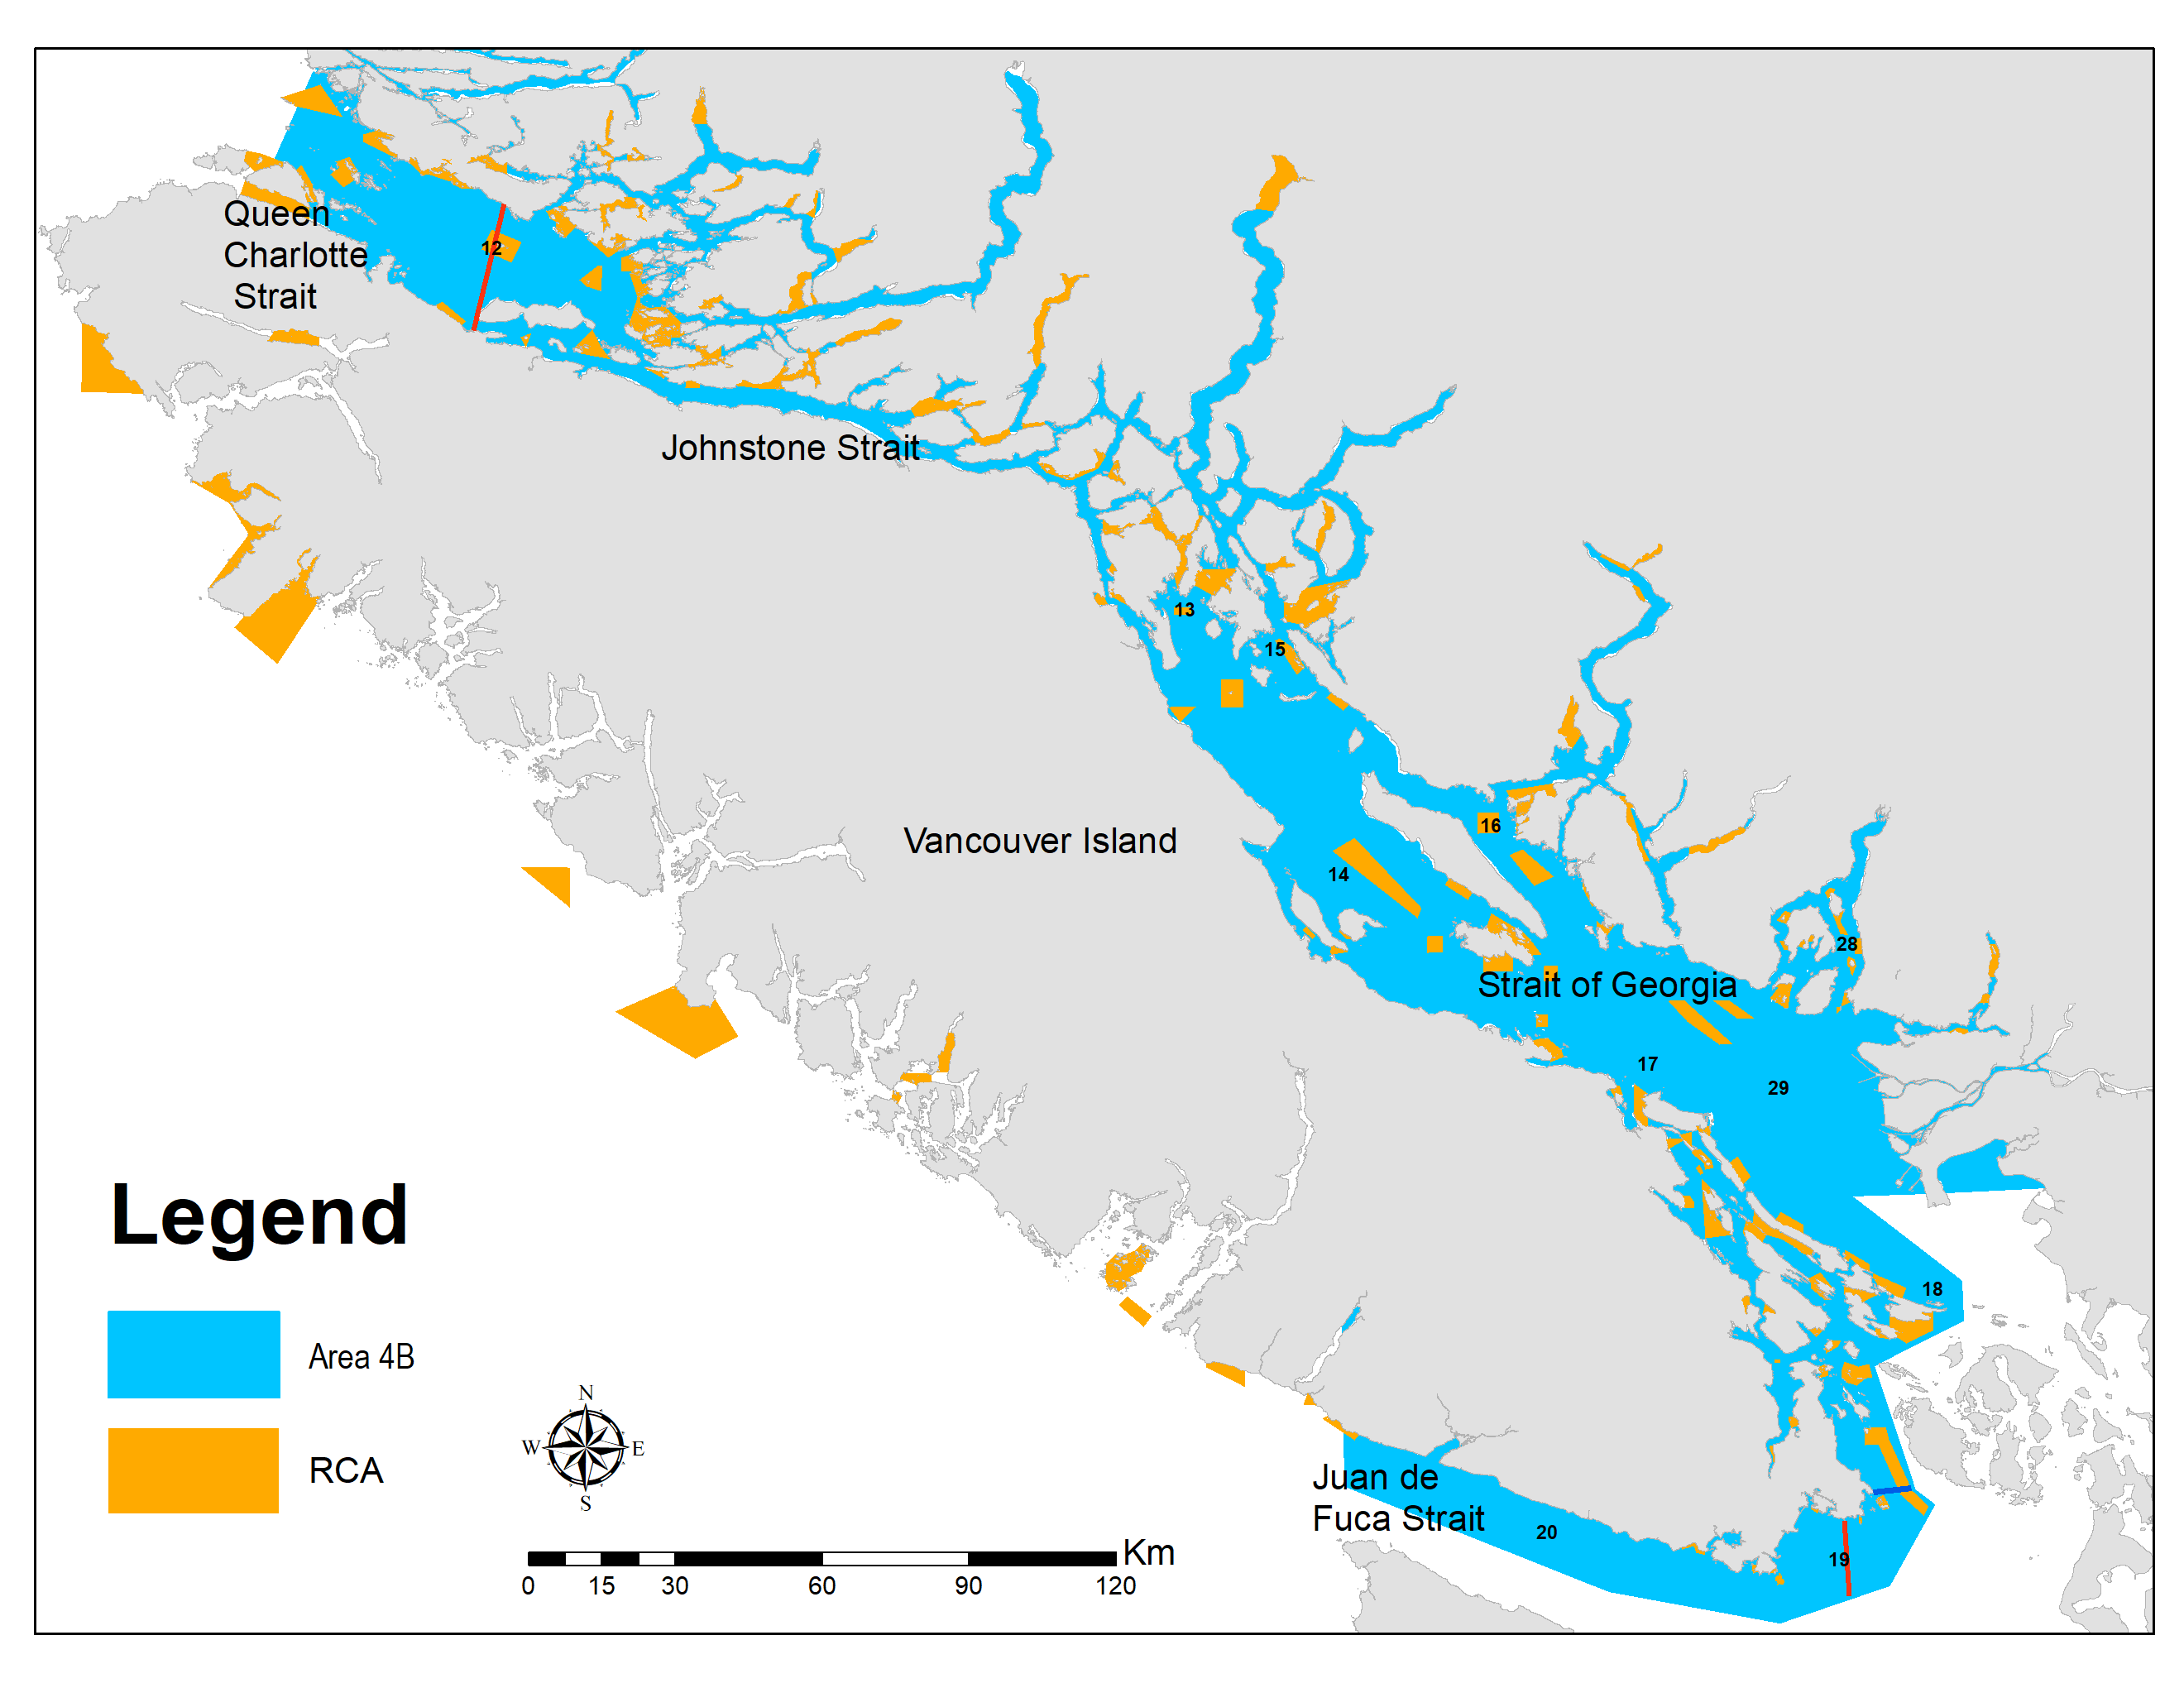
\includegraphics[width=5in]{C:/GitHub/yelloweye-inside/figs-french/InsideYE_Map_new}}{Figure \ref{fig:map-4B}} 

}

\caption{Carte de la zone de gestion 4B du poisson de fond montrant les aires de conservation du sébaste (ACS) et les limites séparant l'unité désignable (UD) du sébaste aux yeux jaunes des eaux intérieures de l'UD du sébaste aux yeux jaunes des eaux extérieures. Les lignes rouges indiquent une proposition d'ajustement de l'aire de répartition de l'UD des eaux intérieures, fondée sur des preuves génétiques récentes (Siegle \protect\hyperlink{ref-siegle2011}{2011}; Siegle et al. \protect\hyperlink{ref-siegle2013}{2013}; Andrews et al. \protect\hyperlink{ref-andrews2018}{2018}).}\label{fig:map-4B}
\end{figure}
L'objectif du plan de rétablissement actuel est de « reconstituer le stock au-dessus du PRL sur 80 ans avec une probabilité de réussite de 56 \% ». Le jalon cible est de « dégager des tendances positives au cours de chaque période de 10 ans ». La procédure de gestion actuelle du sébaste aux yeux jaunes des eaux intérieures vise à maintenir les prises annuelles totales (commerciales, récréatives, alimentaires, sociales et rituelles des Premières Nations et de relevé) à moins de 15 tonnes (voir l'annexe 9 du document DFO (\protect\hyperlink{ref-ifmp2018}{2018}) pour plus de renseignements).

D'après les directives, les plans de rétablissement au Canada doivent présenter une forte probabilité de rétablissement des stocks de poissons hors de la zone critique dans le délai prescrit (MPO \protect\hyperlink{ref-dfo2013}{2013}). Ce projet vise notamment à répondre à une préoccupation exprimée par les gestionnaires des pêches, à savoir que la probabilité de réussite de 56 \% énoncée dans le plan de rétablissement actuel (DFO \protect\hyperlink{ref-ifmp2018}{2018}) ne correspond pas à la définition d'une probabilité élevée.

Le document d'orientation indique également certaines mesures de gestion recommandées, comme le maintien des prélèvements par toutes les sources au niveau le plus bas possible, l'élaboration d'une règle de contrôle des prises et l'application de l'évaluation de la stratégie de gestion pour évaluer, par simulation, le rendement d'autres mesures de gestion pour atteindre les objectifs de rétablissement du stock (MPO \protect\hyperlink{ref-dfo2013}{2013}). Le plan de rétablissement actuel met en œuvre un total autorisé des captures annuel fixe de 15 tonnes (DFO \protect\hyperlink{ref-ifmp2018}{2018}), qui n'a pas été mis à l'essai par simulation.

Le sébaste aux yeux jaunes est une espèce qui vit longtemps (jusqu'à 121 ans en Colombie-Britannique, Keppel et Olsen \protect\hyperlink{ref-keppel2019}{2019}), dans des habitats démersaux rocheux répartis de manière irrégulière et discontinue sur la côte intérieure de la Colombie-Britannique (Yamanaka et al. \protect\hyperlink{ref-yamanaka2011}{2011}). Ces caractéristiques du cycle biologique rendent l'espèce vulnérable à la surexploitation par la pêche. Le stock des eaux intérieures est considéré comme étant à données limitées, car peu de données sont accessibles sur la composition selon l'âge, on manque de données biologiques sur les pêches commerciales, récréatives et des Premières Nations, et une incertitude entoure l'ampleur des prises historiques.

\hypertarget{sec:introduction-mse}{%
\subsection{ÉVALUATION DE LA STRATÉGIE DE GESTION}\label{sec:introduction-mse}}

À l'échelle mondiale, la fourniture d'avis scientifiques pour la gestion des pêches a évolué vers des approches axées sur l'évaluation de la stratégie de gestion (ou axées sur la gestion) (p.~ex., Butterworth et Punt \protect\hyperlink{ref-butterworth1999}{1999}; Rademeyer et al. \protect\hyperlink{ref-rademeyer2007}{2007}; Berkson et Thorson \protect\hyperlink{ref-berkson2015}{2015}; Geromont et Butterworth \protect\hyperlink{ref-geromont2015}{2015}; Carruthers et al. \protect\hyperlink{ref-carruthers2016}{2016}; Punt et al. \protect\hyperlink{ref-punt2016}{2016}). L'évaluation de la stratégie de gestion se concentre sur la détermination des procédures de gestion qui donnent les meilleurs résultats en ce qui concerne l'atteinte des objectifs convenus en matière de politique et de pêche, lorsqu'ils sont mis en œuvre dans un environnement de simulation en « boucle fermée » (figure~\ref{fig:mse-chart-basic}). Dans les pêches à production contrôlée, comme la pêche du poisson de fond en Colombie-Britannique, où les quotas sont gérés, les procédures de gestion décrivent les mesures de gestion pour l'établissement des limites des prises. Les données exigées dans les procédures de gestion peuvent varier considérablement, allant d'approches très riches en données, y compris les évaluations statistiques des prises selon l'âge avec des règles de contrôle des prises, à des règles de données simples (approches « limitées en données »), qui ne reposent que sur les données sur les prises et un indice de l'abondance (p.~ex., Geromont et Butterworth \protect\hyperlink{ref-geromont2015}{2015}; Carruthers et al. \protect\hyperlink{ref-carruthers2016}{2016}).

La simulation en boucle fermée diffère des approches d'évaluation classique des stocks parce qu'elle simule la rétroaction entre la mise en œuvre des procédures de gestion et le système sous-jacent (le stock de poisson et son environnement), décrite par un ou plusieurs modèles opérationnels. L'approche de la simulation en boucle fermée tient compte de l'effet des procédures de gestion sur le système, ainsi que des données futures recueillies dans le système et de leur utilisation chez les procédures de gestion (Punt et al. \protect\hyperlink{ref-punt2016}{2016}; Carruthers et Hordyk \protect\hyperlink{ref-carruthers2018}{2018}\protect\hyperlink{ref-carruthers2018}{a}; Anderson et al. \protect\hyperlink{ref-anderson2020gfmp}{2020}\protect\hyperlink{ref-anderson2020gfmp}{b}).


\begin{figure}[htb]

{\centering \pdftooltip{\includegraphics[width=6.3in]{C:/GitHub/yelloweye-inside/figs-french/mse-chart-simple2}}{Figure \ref{fig:mse-chart-basic}} 

}

\caption{Illustration du processus de simulation en boucle fermée des pêches d'après Anderson et al. (\protect\hyperlink{ref-anderson2020gfmp}{2020}\protect\hyperlink{ref-anderson2020gfmp}{b}), selon Punt et al. (\protect\hyperlink{ref-punt2016}{2016}). La procédure de gestion peut être fondée sur une règle de données simple (p.~ex., réduire les prises autorisées de x \% si l'indice du relevé diminue de y \%) ou peut être un modèle d'estimation combiné à une règle de contrôle des prises.}\label{fig:mse-chart-basic}
\end{figure}
\hypertarget{sec:introduction-approach}{%
\subsection{APPROCHE}\label{sec:introduction-approach}}

En raison des données limitées sur le stock de sébaste aux yeux jaunes des eaux intérieures, il est difficile d'évaluer le rendement prévu des mesures de gestion nécessaires pour rendre le stock conforme aux dispositions sur les stocks de poissons, c.-à-d.~pour le faire sortir de la zone critique dans le délai convenu et avec la probabilité convenue. La simulation-mise à l'essai en boucle fermée des procédures de gestion à données limitées permet d'évaluer le rendement relatif des procédures de gestion dans un éventail d'incertitudes entourant, par exemple, la biologie sous-jacente des poissons, l'erreur d'observation, l'erreur d'estimation et l'erreur de mise en œuvre (p.~ex., Kell et al. \protect\hyperlink{ref-kell2006}{2006}; Carruthers et al. \protect\hyperlink{ref-carruthers2016}{2016}).

Depuis 2017, une entente de partenariat entre l'Université de la Colombie-Britannique et le MPO (DFO \protect\hyperlink{ref-dfo_dlmtool_2017}{2017}) a facilité l'élaboration de deux progiciels à accès libre pour l'évaluation de la stratégie de gestion, mis en œuvre dans l'environnement de programmation statistique R (R Core Team \protect\hyperlink{ref-r2019}{2019})~: l'outil pour les méthodes à données limitées (DLMtool) (Carruthers et Hordyk \protect\hyperlink{ref-carruthers2018}{2018}\protect\hyperlink{ref-carruthers2018}{a}, \protect\hyperlink{ref-carruthers_hordyk_2018}{2018}\protect\hyperlink{ref-carruthers_hordyk_2018}{b}) et l'outil pour l'évaluation de la stratégie de gestion (MSEtool) (Huynh et al. \protect\hyperlink{ref-huynh_msetool_2019}{2019}). Après plusieurs années de développement, ces progiciels sont parmi les logiciels les plus rapides, les plus souples et les plus extensibles pour évaluer les stratégies de gestion des pêches. Ils peuvent être appliqués à des stocks pauvres ou riches en données, permettant d'évaluer rapidement plusieurs procédures de gestion en fonction d'objectifs de conservation et de pêche personnalisables, et d'évaluer les principaux compromis.

\hypertarget{sec:introduction-mp-framework}{%
\subsubsection{Cadre des procédures de gestion du poisson de fond en Colombie-Britannique}\label{sec:introduction-mp-framework}}

Le Cadre des procédures de gestion pour le poisson de fond en Colombie-Britannique (Anderson et al. \protect\hyperlink{ref-anderson2020gfmp}{2020}\protect\hyperlink{ref-anderson2020gfmp}{b}) a été élaboré parallèlement au présent document pour évaluer le rendement d'un large éventail de procédures de gestion pour les espèces de poisson de fond à données limitées. Le Cadre des procédures de gestion fait largement appel aux fonctions de DLMtool et de MSEtool, avec l'appui d'un progiciel R gfdlm (Anderson et al. \protect\hyperlink{ref-gfdlm}{2020}\protect\hyperlink{ref-gfdlm}{d}) rédigé par les auteurs de Anderson et al. (\protect\hyperlink{ref-anderson2020gfmp}{2020}\protect\hyperlink{ref-anderson2020gfmp}{b}), qui contient un ensemble d'outils de soutien logiciel et des visualisations personnalisées.

Nous suivons le Cadre des procédures de gestion pour sélectionner les procédures de gestion afin d'établir des limites des prises pour les stocks de poissons de fond à données limitées (Anderson et al. \protect\hyperlink{ref-anderson2020gfmp}{2020}\protect\hyperlink{ref-anderson2020gfmp}{b}). Notre évaluation du plan de rétablissement du sébaste aux yeux jaunes des eaux intérieures constitue la première application du Cadre des procédures de gestion pour produire un avis scientifique à l'appui des décisions sur les prises. Le cadre suit six étapes de pratiques exemplaires décrites ci-après et plus en détail dans Anderson et al. (\protect\hyperlink{ref-anderson2020gfmp}{2020}\protect\hyperlink{ref-anderson2020gfmp}{b}).

Les étapes des pratiques exemplaires sont fondées sur un examen effectué par Punt et al. (\protect\hyperlink{ref-punt2016}{2016}), qui a cerné cinq étapes clés du processus d'évaluation de la stratégie de gestion (étapes 2 à 6 ci-après). Une première étape supplémentaire du Cadre des procédures de gestion, qui définit le contexte décisionnel, a été définie par Gregory et al. (\protect\hyperlink{ref-gregory2012}{2012}) et Cox et Benson (\protect\hyperlink{ref-cox2016}{2016}). En grande partie, le logiciel DLMtool a été conçu pour permettre aux praticiens de suivre ces étapes (figure~\ref{fig:mse-chart}; Carruthers et Hordyk \protect\hyperlink{ref-carruthers2018}{2018}\protect\hyperlink{ref-carruthers2018}{a}).



Les six étapes sont les suivantes~:

Étape 1~: Définition du contexte décisionnel.

Étape 2~: Choix des objectifs et des paramètres de rendement.

Étape 3~: Choix des incertitudes/spécification des modèles opérationnels.

Étape 4~: Détermination des procédures de gestion possibles.

Étape 5~: Simulation de l'application des procédures de gestion.

Étape 6~: Présentation des résultats et choix de la procédure de gestion.

\clearpage
\begin{figure}[htb]

{\centering \pdftooltip{\includegraphics[width=\textwidth]{C:/GitHub/yelloweye-inside/figs-french/mse-chart}}{Figure \ref{fig:mse-chart}} 

}

\caption{Les étapes du processus d'évaluation de la stratégie de gestion selon Punt et al. (\protect\hyperlink{ref-punt2016}{2016}), tel que mis en œuvre dans DLMtool. Copié de Anderson et al. (\protect\hyperlink{ref-anderson2020gfmp}{2020}\protect\hyperlink{ref-anderson2020gfmp}{b}) et adapté de Carruthers et Hordyk (\protect\hyperlink{ref-carruthers2018}{2018}\protect\hyperlink{ref-carruthers2018}{a}). Cette figure complète la figure~\ref{fig:mse-chart-basic}.}\label{fig:mse-chart}
\end{figure}
Après la sélection et la mise en œuvre de la procédure de gestion pour l'établissement de la limite des prises (figure~\ref{fig:mse-chart}; par exemple, application de l'algorithme de la procédure de gestion sélectionnée à l'indice du relevé observé), la dernière étape nécessaire consiste à surveiller et à évaluer périodiquement le rendement de la procédure de gestion (MPO \protect\hyperlink{ref-dfo2013}{2013}; Dowling et al. \protect\hyperlink{ref-dowling2015a}{2015}; Carruthers et Hordyk \protect\hyperlink{ref-carruthers2018}{2018}\protect\hyperlink{ref-carruthers2018}{a}). Cela peut se faire par des moyens informels, comme à l'aide de la rétroaction des pêcheurs et des données des relevés (p.~ex., Cox et Kronlund \protect\hyperlink{ref-cox2008a}{2008}), ou au moyen de mesures statistiques plus formelles, où l'on compare les données observées aux prévisions des modèles opérationnels pour vérifier si le système fonctionne comme prévu (Butterworth \protect\hyperlink{ref-butterworth2008}{2008}; Carruthers et Hordyk \protect\hyperlink{ref-carruthers_hordyk_2018}{2018}\protect\hyperlink{ref-carruthers_hordyk_2018}{b}; discussion dans Anderson et al. \protect\hyperlink{ref-anderson2020gfmp}{2020}\protect\hyperlink{ref-anderson2020gfmp}{b}).

Dans les sections suivantes, nous décrivons notre approche pour l'élaboration d'un éventuel plan de rétablissement du sébaste aux yeux jaunes des eaux intérieures, en suivant les six étapes des pratiques exemplaires.

\section{DONNÉES DES RELEVÉS INDÉPENDANTES DE LA PÊCHE}
\label{app:index-data}

Nous avons conditionné les modèles opérationnels à l'aide d'indices de l'abondance tirés du relevé à la palangre sur fond dur (RPFD) et du relevé à la palangre sur l'aiguillat commun dans le détroit de Georgie. Les plans de relevé et la modélisation des indices connexes sont décrits ici.

\hypertarget{sec:hbll-index-data}{%
\subsection{INDICE DU RELEVÉ À LA PALANGRE SUR FOND DUR DANS LES EAUX INTÉRIEURES}\label{sec:hbll-index-data}}

Le relevé à la palangre sur fond dur dans les eaux intérieures pour la zone de gestion du détroit de Georgie (4B) fournit des indices des taux de prise et les données biologiques connexes pour l'évaluation du sébaste des zones côtières depuis 2003 (Lochead et Yamanaka \protect\hyperlink{ref-lochead2007}{2007}). Le relevé suit un plan stratification aléatoire de la profondeur qui consiste en blocs de 2 km par 2 km, et il a toujours été effectué par le NGCC Neocaligus. Le relevé utilise des hameçons circulaires de type agrafe de taille 13/0 et du calmar comme appât avec une durée d'immersion de deux heures. Les données hameçon par hameçon recueillies depuis le début des relevés sont collectées électroniquement et stockées dans une base de données. Pour plus de renseignements détaillés sur le plan du relevé, voir Lochead et Yamanaka (\protect\hyperlink{ref-lochead2004}{2004}).

La zone du relevé est divisée en régions du nord et du sud (figure~\ref{fig:map-HBLL-NS}), qui sont pêchées en alternance une année sur deux. La frontière entre les deux régions se situe approximativement aux extrémités nord des secteurs de gestion des pêches du Pacifique (SGPP) 14 et 15 (figure~\ref{fig:map-4B}). Cependant, plusieurs irrégularités se sont produites (figure~\ref{fig:hbll-raw})~:


\begin{figure}[htb]

{\centering \pdftooltip{\includegraphics[width=5in]{C:/GitHub/yelloweye-inside/figs-french/YE_Inside_2019_HBLL_L}}{Figure \ref{fig:map-HBLL-NS}} 

}

\caption{Carte des blocs du relevé à la palangre sur fond dur indiquant les régions du nord (en bleu) et du sud (en vert). Les aires de conservation du sébaste (blocs orange) sont également représentées.}\label{fig:map-HBLL-NS}
\end{figure}
\begin{itemize}

\item
  Le relevé n'a pas eu lieu en 2006 et en 2017.
\item
  La durée du relevé varie d'une année à l'autre, ce qui se traduit par des incohérences dans la portée géographique du relevé d'une année à l'autre.
\item
  La baie Desolation (SGPP 15) fait partie de la région du sud, mais a été échantillonnée dans la région du nord en 2003, 2008 et 2019, et ne l'a pas été en 2009 et 2018. Les taux de prise du sébaste aux yeux jaunes sont les plus élevés dans la baie Desolation (SGPP 15; figure~\ref{fig:map-4B}). Le manque d'échantillonnage en 2009 et en 2018 devrait donc avoir un effet sur les estimations du relevé du sud.
\item
  Le relevé du sud n'a pas été réalisé en entier en 2009; la pêche a seulement eu lieu dans 38 blocs dans le sud du détroit de Georgie, et uniquement entre Nanaimo et Victoria. Cela contraste avec les années normales où le relevé couvre environ 70 blocs jusqu'à Campbell River au nord. Les taux de prise de la plupart des espèces de sébastes capturées dans ce relevé ayant tendance à diminuer du nord au sud, cela pourrait également avoir un effet important sur l'indice du relevé cette année-là.
\end{itemize}
Nous avons appliqué un modèle spatiotemporel géostatistique pour normaliser l'indice du relevé à la palangre sur fond dur (p.~ex., Shelton et al. \protect\hyperlink{ref-shelton2014}{2014}; Thorson et al. \protect\hyperlink{ref-thorson2015}{2015}; Anderson et al. \protect\hyperlink{ref-anderson2019synopsis}{2019}) afin de tenir compte de la mise en œuvre irrégulière du plan du relevé (section~\ref{sec:hbll-spatiotemporal}). Nous avons confirmé, par simulation, que cette approche peut « assembler » les régions de relevé du nord et du sud avec relativement peu de biais (section~\ref{sec:hbll-sim}).

\hypertarget{sec:hbll-hook-competition}{%
\subsubsection{Concurrence à l'hameçon}\label{sec:hbll-hook-competition}}

Un indice de l'abondance d'une espèce tiré d'un relevé à la palangre n'est pas forcément proportionnel à l'abondance réelle dans certaines conditions. Par exemple, en cas de forte concurrence entre les espèces pour les hameçons appâtés, les prises réelles pourraient ne pas refléter fidèlement la véritable abondance des espèces moins compétitives (Kuriyama et al. \protect\hyperlink{ref-kuriyama2018}{2018}). Les prises du relevé à la palangre sur fond dur dans les eaux intérieures sont principalement composées d'aiguillat commun du Pacifique Nord (\emph{Squalus suckleyi}; ci-après « aiguillat commun »), un important concurrent potentiel des sébastes aux hameçons (Obradovich \protect\hyperlink{ref-obradovich2018}{2018}). Comme dans Yamanaka et al. (\protect\hyperlink{ref-yamanaka2011}{2011}), nous avons appliqué une correction de la concurrence à l'hameçon, qui tient compte de la concurrence entre les poissons individuels pour l'appât des hameçons, aux données du relevé à la palangre sur fond dur. Pour appliquer cette correction, on estime un facteur d'ajustement de la concurrence pour chaque calée, chaque année. Ce facteur d'ajustement, \(A_{i,t}\), met à l'échelle le nombre observé de sébastes aux yeux jaunes capturés, \(N_{i,t}\), pour chaque calée \(i\) chaque année \(t\) afin de donner le nombre prévu de poissons pêchés après la prise en compte de la concurrence, \(N_{i,t}^{(0)}\)~:
\begin{equation}
N_{i,t}^{(0)} = A_{i,t} N_{i,t}.
\label{eq:Nit}
\end{equation}
Le facteur d'ajustement dépend de la proportion d'hameçons observés qui sont remontés encore appâtés, \(P_{i,t}\) (figure~\ref{fig:hbll-baited})~:
\begin{equation}
A_{i,t} = – \frac{ \log P_{i,t}}{1 – P_{i,t}}.
\label{eq:hbll-hook-adjustment}
\end{equation}
Étant donné que \(P_{i,t} \rightarrow 0\), \(A_{i,t} \rightarrow \infty\), de sorte que le nombre prévu \(N_{i,t}^{(0)} \rightarrow \infty\). Par conséquent, dans les cas où aucun hameçon n'a été remonté encore appâté, nous avons fixé le nombre d'hameçons appâtés à un. Voir plus de renseignements détaillés sur la correction de la concurrence à l'hameçon dans Anderson et al. (\protect\hyperlink{ref-anderson2019synopsis}{2019}) (leur annexe G, section G.5). Nous avons entré les données ajustées en fonction de la concurrence à l'hameçon (figure~\ref{fig:hbll-hook-adjustment}) dans le modèle spatiotemporel pour développer l'indice de l'abondance.

\hypertarget{sec:hbll-spatiotemporal}{%
\subsubsection{Normalisation de l'indice spatiotemporel du relevé à la palangre sur fond dur}\label{sec:hbll-spatiotemporal}}

Nous avons ajusté un modèle de normalisation de l'indice spatiotemporel géostatistique~:
\begin{align}
  y_{s,t} &\sim \mathrm{NegBin}\left(\mu_{s,t}, \phi \right),\\
  \mu_{s,t} &= \exp \left( \bm{X}_{s,t} O_{s,t} + \bm{\beta} + \omega_s + \epsilon_{s,t} \right),
\label{eq:hbll-model}
\end{align}
où NegBin fait référence à la distribution binomiale négative (le paramétrage NB2 (Hilbe \protect\hyperlink{ref-hilbe2011}{2011}) où les échelles de la variance sont en quadrature avec la moyenne), \(\phi\) représente le paramètre de dispersion, \(y_{s,t}\) et \(\mu_{s,t}\) font référence à la valeur observée et prévue, respectivement, au point spatial \(s\) et dans le temps \(t\), \(\phi\) désigne le paramètre de dispersion, \(\bm{X}\) désigne une matrice du plan et \(\beta\) désigne un vecteur de coefficients estimés (une moyenne indépendante pour chaque année). Le symbole \(O_{s,t}\) représente une « compensation » pour le nombre d'hameçons et le facteur d'ajustement de la concurrence à l'hameçon. Plus précisément, il était représenté en tant que \(\log \left(S_{i,t} / A_{i,t} \right)\), où \(S_{i,t}\) représente la superficie « balayée » par la calée. Nous avons calculé la superficie balayée en fonction du nombre d'hameçons (\(N^\textrm{hooks}_{i,t}\)) dans la calée \(i\) et l'année \(t\) comme suit~:
\begin{equation}
N^\textrm{hooks}_{i,t} \cdot 0.0024384 \cdot 0.009144 \cdot 1000.
\end{equation}
La valeur 0,002438 correspond à l'espacement entre les hameçons (8 pouces) en kilomètres, 0,009144 à une superficie présumée de 30 pieds balayée autour de la calée où les poissons peuvent être capturés (en kilomètres) et 1 000 met à l'échelle la superficie balayée des kilomètres aux mètres. Il est à noter que l'hypothèse de 30 pieds ne sert qu'à augmenter ou à diminuer la densité pour toutes les années et a en fin de compte une incidence sur l'estimation de la capturabilité du relevé, mais n'influencera pas la forme des séries chronologiques de l'indice.

Nous avons supposé que les effets aléatoires spatiaux (\(\omega_s\)) étaient tirés d'une distribution normale multidimensionnelle avec une matrice de covariance \(\bm{\Sigma}_\omega\)~:
\begin{equation}
\bm{\omega} \sim \mathrm{MVNormal} \left( \bm{0}, \bm{\Sigma}_\omega \right).
\end{equation}
Nous avons limité les effets aléatoires spatiaux pour suivre une fonction de covariance de \mbox{Mat\'ern}, qui définit le taux de décroissance de la corrélation spatiale avec la distance. La fonction de \mbox{Mat\'ern} décrit la covariance \(\Phi_\omega \left( s_j, s_k \right)\) entre les emplacements spatiaux \(s_j\) et \(s_k\) comme suit~:
\begin{equation}
\Phi_\omega\left( s_j,s_k \right) = \tau_\omega^2/\Gamma(\nu)2^{\nu – 1}
    (\kappa d_{jk})^\nu K_\nu \left( \kappa d_{jk} \right),
\end{equation}
où \(\tau_\omega^2\) représente la variance spatiale, \(\Gamma\) représente la fonction gamma, \(K_\nu\) représente la fonction de Bessel, \(d_{jk}\) représente la distance euclidienne entre les emplacements \(s_j\) et \(s_k\), et \(\kappa\) représente un paramètre d'échelle estimé (p.~ex., Lindgren et al. \protect\hyperlink{ref-lindgren2011}{2011}). Le paramètre \(\nu\) contrôle le lissage de la fonction de covariance. Nous avons établi \(\nu = 1\), ce qui nous permet de tirer parti de l'approximation de l'équation différentielle partielle stochastique (SPDE) aux champs aléatoires de Markov gaussien (GMRF) pour augmenter considérablement l'efficacité de calcul (Lindgren et al. \protect\hyperlink{ref-lindgren2011}{2011}).

Nous avons supposé la même structure pour les effets aléatoires spatiotemporels, en attribuant à chaque tranche de temps son propre ensemble indépendant d'effets aléatoires (\(\bm{\epsilon}_t\)) avec la matrice de covariance \(\bm{\Sigma}_{\epsilon,t}\)~:
\begin{equation}
\bm{\epsilon}_t \sim \mathrm{MVNormal} \left( \bm{0}, \bm{\Sigma}_{\epsilon,t} \right).
\end{equation}
Cette matrice de covariance est également limitée pour suivre une fonction de covariance de \mbox{Mat\'ern} avec le même \(\kappa\), mais son propre \(\tau_\epsilon^2\) (variance spatiale)~:
\begin{equation}
\Phi_\epsilon\left( s_j,s_k \right) = \tau_\epsilon^2/\Gamma(\nu)2^{\nu – 1}
    (\kappa d_{jk})^\nu K_\nu \left( \kappa d_{jk} \right).
\end{equation}
Bien que nous ayons décrit les fonctions de \mbox{Mat\'ern} ci-dessus en utilisant la forme isométrique simple dans un souci de simplicité (la corrélation spatiale est la même dans toutes les directions), nous avons en fait autorisé l'anisotropie dans la corrélation spatiale et spatiotemporelle (p.~ex., Thorson et al. \protect\hyperlink{ref-thorson2015}{2015}).

Les effets aléatoires spatiaux tenaient compte de facteurs spatiaux qui étaient constants dans le temps, comme la profondeur et le type de substrat. Les effets aléatoires spatiotemporels intégraient des facteurs qui variaient d'une année à l'autre dans l'espace, comme la température au fond, les régimes de circulation de l'eau, les interactions entre espèces et les déplacements des espèces. À titre d'analyses de sensibilité, nous avons inclus d'autres versions de nos modèles qui 1) tenaient également compte de la profondeur et 2) ne tenaient pas compte de la concurrence à l'hameçon.

Nous avons ajusté notre modèle avec le progiciel sdmTMB en R (Anderson et al. \protect\hyperlink{ref-sdmtmb}{2020}\protect\hyperlink{ref-sdmtmb}{a}) et TMB (Kristensen et al. \protect\hyperlink{ref-tmb}{2016}) en utilisant un « maillage » avec 400 « nœuds » de processus prédictifs générés par des approximations de Laplace imbriquées et intégrées (INLA) (Lindgren et al. \protect\hyperlink{ref-lindgren2011}{2011}; Rue et al. \protect\hyperlink{ref-rue2016}{2016}) avec des emplacements déterminés par un algorithme de regroupement des K-moyennes (figure~\ref{fig:hbll-spde}). Nous avons estimé les effets fixes par vraisemblance maximale, les effets aléatoires étant fixés aux valeurs qui maximisaient la probabilité conjointe conditionnelle à la valeur estimée des effets fixes. Nous avons vérifié que les ajustements du modèle concordaient avec la convergence en nous assurant que le gradient maximal de tous les coefficients estimés était inférieur à 0,001 et que la matrice de covariance était positive-définie.

Nous avons projeté les prévisions du modèle sur toute la zone de relevé (figure~\ref{fig:hbll-area-grid}) à l'aide de la matrice de projection de covariance et du maillage d'interpolation bilinéaire fournis par INLA (Lindgren et al. \protect\hyperlink{ref-lindgren2011}{2011}; Rue et al. \protect\hyperlink{ref-rue2016}{2016}) (figures~\ref{fig:hbll-spde} et~\ref{fig:hbll-predicted-spacetime}). En ce qui concerne les composantes du modèle, les effets aléatoires spatiaux étaient, par définition, constants d'une année à l'autre (figure~\ref{fig:hbll-spatial-re}) et les effets aléatoires spatiotemporels variaient d'une année à l'autre (figure~\ref{fig:hbll-spatiotemporal-re}).

Nous avons alors calculé la biomasse prévue \(B_t\) pour l'année \(t\), comme suit~:
\begin{equation}
B_t = \sum_{j = 1}^{n_j}
  w_j \cdot \exp \left( \bm{X}_{j,t} \bm{\beta} + \bar{\bm{O}} + \omega_j + \epsilon_{j,t} \right),
\end{equation}
où \(j\) renvoie à une cellule du quadrillage dans la zone de relevé, \(w_j\) représente la superficie de cette cellule (figure~\ref{fig:hbll-area-grid}) et \(\bar{\bm{O}}\) représente la valeur de compensation moyenne. En d'autres termes, nous avons additionné la biomasse prévue pour chaque année dans toutes les cellules de quadrillage faisant partie de la zone de relevé. Nous avons généré les écarts­types pour les estimations annuelles de la biomasse logarithmique à l'aide de la méthode delta généralisée mise en œuvre dans Template Model Builder (Kristensen et al. \protect\hyperlink{ref-tmb}{2016}).

L'indice de la population normalisé ainsi obtenu tient compte de l'échantillonnage irrégulier de la zone de relevé et de la concurrence à l'hameçon et « assemble » les régions du nord et du sud en un seul indice de la population (figure~\ref{fig:hbll-index}). L'inclusion de la profondeur ou l'exclusion des ajustements de la concurrence à l'hameçon ont eu des effets relativement mineurs sur l'indice de la population (figure~\ref{fig:hbll-index}). Le modèle a également été en mesure de « remplir » ce à quoi l'indice pourrait ressembler hypothétiquement pour les régions du nord et du sud indépendamment (figure~\ref{fig:hbll-index}). Il convient de noter que cette interpolation statistique ne peut pas tenir compte d'événements ponctuels dans la région non observée, comme une abondance anormalement élevée seulement dans la région du nord une année où le relevé avait lieu dans la région du sud.

\hypertarget{sec:hbll-sim}{%
\subsubsection{Essais par simulation de « l'assemblage » des relevés par les modèles spatiotemporels}\label{sec:hbll-sim}}

Nous avons entrepris une analyse de simulation de base pour vérifier que notre approche « d'assemblage » des régions du nord et du sud dans une seule zone de relevé était raisonnable d'un point de vue statistique. Nous avons produit un système qui correspond approximativement aux données du relevé à la palangre sur fond dur avec lesquelles nous avons travaillé dans ce document~:
\begin{itemize}

\item
  10 ans d'observations
\item
  100 emplacements d'observation spatiale possibles, \(s_j\) et \(s_k\), tirés d'une distribution uniforme (0, 1) chaque année
\item
  Un ET marginal (\(\omega_s\)) = 2,2
\item
  Un ET marginal (\(\epsilon_{s,t}\)) = 0,3
\item
  Un paramètre de \mbox{Mat\'ern} \(\kappa = 0,1\)
\item
  Des moyennes annuelles tirées d'une distribution log-normale (0,1, 0,2)
\item
  Un processus d'observation de Poisson (dans un souci de simplicité plutôt qu'un binôme négatif)
\end{itemize}
Nous avons simulé l'abondance moyenne réelle sous-jacente sur un quadrillage complet {[}0, 1{]} contenant 25 x 25 cellules de taille égale. Nous avons ensuite rejeté les régions du nord et du sud (au-dessus ou en dessous de 0,5) en alternance une année sur deux, afin d'avoir environ 50 observations par année, et nous avons tenté d'ajuster la même forme de modèle spatiotemporel que celle utilisée pour la normalisation de l'indice du relevé à la palangre sur fond dur (figure~\ref{fig:stich-sim-pred}).

Même s'il n'observait que les régions du nord et du sud en alternance, le modèle a été en mesure de reconstituer les parties manquantes non observées à partir de la corrélation spatiale estimée et, dans une moindre mesure, de la corrélation spatiotemporelle estimée (figure~\ref{fig:stich-sim-pred}). En projetant les prévisions du modèle sur un quadrillage de toute la superficie du carré simulé, notre modèle a pu produire un indice semblable à l'indice réel (figure~\ref{fig:stich-sim-index}). Si nous générions plutôt l'indice de façon naïve en utilisant une approche qui imite une approche fondée sur le plan (en additionnant les abondances observées chaque année et en l'ajustant à la même moyenne géométrique à des fins de visualisation), l'indice obtenu ne reflétait pas la tendance de l'indice réel pour beaucoup d'années (figure~\ref{fig:stich-sim-index}).

Grâce à l'expérimentation (non illustrée), nous avons constaté que « l'assemblage » était le plus exact pour récupérer l'indice réel si l'ampleur des écarts de la corrélation spatiale (\(\omega_s\)) était beaucoup plus grande que celle des écarts de la corrélation spatiotemporelle (\(\epsilon_{s,t}\)). C'est le cas dans notre modèle de relevé à la palangre sur fond dur, où l'écart-type marginal de \(\omega_s\) était environ six fois plus grand que l'écart-type marginal de \(\epsilon_{s,t}\). « L'assemblage » était le plus nécessaire lorsque l'abondance présentait un gradient nord-sud, comme cela semble évident pour le sébaste aux yeux jaunes.
\begin{figure}[htb]

{\centering \pdftooltip{\includegraphics[width=\textwidth]{C:/GitHub/yelloweye-inside/figs-french/hbll-joint-raw-data}}{Figure \ref{fig:hbll-raw}} 

}

\caption{Observations de sébaste aux yeux jaunes dans le relevé à la palangre sur fond dur dans les eaux intérieures. L’arrière-plan ombré en gris indique les zones de relevé du nord et du sud. La superficie des cercles représente le nombre de poissons capturés par hameçon après prise en compte de la concurrence à l’hameçon.}\label{fig:hbll-raw}
\end{figure}
\begin{figure}[htb]

{\centering \pdftooltip{\includegraphics[width=5in]{C:/GitHub/yelloweye-inside/figs-french/hbll-area-in-water}}{Figure \ref{fig:hbll-area-grid}} 

}

\caption{Superficie par cellule de quadrillage du relevé qui se trouve dans l’eau pour le relevé à la palangre sur fond dur dans les eaux intérieures. La densité de comptage prévue pour chaque cellule du quadrillage est étendue à toute la zone de relevé en fonction de ces régions.}\label{fig:hbll-area-grid}
\end{figure}
\begin{figure}[htb]

{\centering \pdftooltip{\includegraphics[width=\textwidth]{C:/GitHub/yelloweye-inside/figs-french/hbll-joint-baited}}{Figure \ref{fig:hbll-baited}} 

}

\caption{Proportion d’hameçons appâtés remontés pour le relevé à la palangre sur fond dur dans les eaux intérieures. Il convient de noter la différence importante entre les régions du nord et du sud et le changement dans le nord entre 2003 et 2007 et les années suivantes.}\label{fig:hbll-baited}
\end{figure}
\begin{figure}[htb]

{\centering \pdftooltip{\includegraphics[width=\textwidth]{C:/GitHub/yelloweye-inside/figs-french/hbll-joint-hook-adjust}}{Figure \ref{fig:hbll-hook-adjustment}} 

}

\caption{Facteur d’ajustement des hameçons pour le relevé à la palangre sur fond dur dans les eaux intérieures, tenant compte du nombre d’hameçons et du nombre d’hameçons remontés appâtés.}\label{fig:hbll-hook-adjustment}
\end{figure}
\begin{figure}[htb]

{\centering \pdftooltip{\includegraphics[width=0.6\textwidth]{C:/GitHub/yelloweye-inside/figs-french/hbll-joint-spde}}{Figure \ref{fig:hbll-spde}} 

}

\caption{Maillage de l’équation différentielle partielle stochastique (SPDE) pour le relevé à la palangre sur fond dur. Les cercles gris ouverts en arrière-plan (souvent masqués) représentent les emplacements des données observées et les points rouges représentent les "knots". Les lignes indiquent le maillage de triangularisation utilisé dans l’approximation de l’équation différentielle partielle stochastique et l’interpolation bilinéaire. Un plus grand nombre de nœuds augmente la précision de l’approximation au détriment du temps de calcul.}\label{fig:hbll-spde}
\end{figure}
\begin{figure}[htb]

{\centering \pdftooltip{\includegraphics[width=\textwidth]{C:/GitHub/yelloweye-inside/figs-french/hbll-joint-prediction-log}}{Figure \ref{fig:hbll-predicted-spacetime}} 

}

\caption{Densité relative prédite dans l’espace et le temps pour le relevé à la palangre sur fond dur. Les nombres observés (avec ajustement des hameçons) sont illustrés par des cercles. Les prédictions sont illustrées par des ombres de couleur.}\label{fig:hbll-predicted-spacetime}
\end{figure}
\begin{figure}[htb]

{\centering \pdftooltip{\includegraphics[width=4.2in]{C:/GitHub/yelloweye-inside/figs-french/hbll-joint-omega}}{Figure \ref{fig:hbll-spatial-re}} 

}

\caption{Les effets spatiaux aléatoires. Il s’agit de différences constantes spatialement corrélées dans l’abondance prévue au fil du temps. Les valeurs sont indiquées dans l’espace des liens (log).}\label{fig:hbll-spatial-re}
\end{figure}
\begin{figure}[htb]

{\centering \pdftooltip{\includegraphics[width=\textwidth]{C:/GitHub/yelloweye-inside/figs-french/hbll-joint-epsilon}}{Figure \ref{fig:hbll-spatiotemporal-re}} 

}

\caption{Les effets aléatoires spatiotemporels. Il s’agit d’écarts spatialement corrélés qui changent dans le temps. Noter le retour à la moyenne dans les combinaisons superficie-année sans données d’échantillonnage. Noter la différence d’ampleur entre les effets aléatoires spatiaux (figure précédente) et ces effets aléatoires spatiotemporels.}\label{fig:hbll-spatiotemporal-re}
\end{figure}
\begin{figure}[htb]

{\centering \pdftooltip{\includegraphics[width=4in]{C:/GitHub/yelloweye-inside/figs-french/hbll-index-components-eps-depth2}}{Figure \ref{fig:hbll-index}} 

}

\caption{L’indice commun de l’abondance relative. Le graphique du haut illustre la prédiction commune à partir du modèle spatial temporel. Trois versions sont incluses~: 1) les effets aléatoires et les moyennes annuelles seulement, 2) l’ajout d’une covariable de profondeur et 3) l’élimination du facteur d’ajustement des hameçons. Les graphiques du milieu et du bas représentent les prévisions communes pour les régions du nord et du sud. Toutes les régions ombrées représentent des intervalles de confiance de 95\%. Les séries chronologiques des indices communs du graphique du haut ont été mises à l’échelle pour avoir la même moyenne géométrique que le principal indice ``RPFD INT'' à des fins de visualisation. Les lignes verticales tiretées indiquent les années où des relevés ont été effectués (surtout) dans la région du sud.}\label{fig:hbll-index}
\end{figure}
\clearpage
\begin{figure}[htb]

{\centering \pdftooltip{\includegraphics[width=\textwidth]{C:/GitHub/yelloweye-inside/figs-french/geostatistical-sim-predicted}}{Figure \ref{fig:stich-sim-pred}} 

}

\caption{Essais par simulation du calcul de l’indice de l’abondance relative avec des observations en alternance pour le nord et le sud. (A) L’abondance réelle simulée (moyenne) dans l’espace et dans le temps. (B) Les nombres observés (points) et estimés (couleurs) dans l’espace et le temps à partir du modèle géostatistique. Les observations se font en alternance une année sur deux dans les régions du nord et du sud et « omettent » la région manquante. Noter comment le modèle temporel spatial est capable de prédire ce que devrait être l’abondance dans la région « omise » en fonction du profil de la corrélation spatiale constante (et, dans une moindre mesure, le profil de la corrélation spatiotemporelle).}\label{fig:stich-sim-pred}
\end{figure}
\clearpage
\begin{figure}[htb]

{\centering \pdftooltip{\includegraphics[width=5in]{C:/GitHub/yelloweye-inside/figs-french/geostatistical-sim-stitched-index}}{Figure \ref{fig:stich-sim-index}} 

}

\caption{Essais par simulation du calcul de l’indice de l’abondance relative avec des observations en alternance pour le nord et le sud. La ligne rouge pleine représente l’abondance réelle simulée dans le temps. La ligne pointillée et tiretée verte représente une estimation « naïve » fondée sur le plan, qui est calculée ici en calculant l’abondance avec seulement les nombres du nord ou du sud observés chaque année. La ligne bleue tiretée représente un indice géostatistique normalisé qui tente de tenir compte des observations biennales nord-sud. La région bleue ombrée représente l’intervalle de confiance de 95\% modélisé.}\label{fig:stich-sim-index}
\end{figure}
\clearpage

\hypertarget{sec:dogfish-index-data}{%
\subsection{INDICE DU RELEVÉ SUR L'AIGUILLAT COMMUN}\label{sec:dogfish-index-data}}

Le relevé sur l'aiguillat commun échantillonne neuf emplacements dans le détroit de Georgie qui ont été historiquement exploités par la pêche commerciale de l'espèce (King et al. \protect\hyperlink{ref-king2012}{2012}). Le relevé a commencé en 1986 et l'échantillonnage a eu lieu en 1989, 2005, 2011, 2014 et 2019. Il s'agit d'un relevé à la palangre stratifié en profondeur qui utilise des engins à agrafe avec 300 hameçons circulaires de taille 14/0 appâtés avec du hareng du Pacifique et une durée d'immersion de deux heures. Une description plus détaillée des méthodes de relevé est donnée dans King et al. (\protect\hyperlink{ref-king2012}{2012}). Pour la plupart des séries chronologiques, les prises de sébaste ont été enregistrées calée par calée. Depuis 2019, des données hameçon par hameçon pour toutes les espèces capturées ont été recueillies à bord, ainsi que les données biologiques pour le sébaste. Nous utilisons un modèle spatiotemporel pour estimer la densité du sébaste aux yeux jaunes par km\textsuperscript{2}. Nous avons calculé la superficie balayée en multipliant le nombre d'hameçons déployés par la distance estimée entre les hameçons (espacement de 8 pieds) et la largeur balayée estimée (longueur de deux avançons).

Le relevé sur l'aiguillat commun n'est pas conçu pour évaluer le sébaste, de sorte qu'il y a plusieurs différences importantes entre les plans des relevés à la palangre sur fond dur et sur l'aiguillat commun. La différence la plus importante est peut-être que le relevé à la palangre sur fond dur cible en particulier les habitats propices au sébaste (c.-à-d.~un fond dur), tandis que le relevé sur l'aiguillat commun est effectuée dans des sites qui étaient importants pour la pêche commerciale et qui présentent principalement des fonds de sédiments meubles. Le relevé sur l'aiguillat commun utilise également des hameçons circulaires légèrement plus gros que ceux utilisés pour le relevé à la palangre sur fond dur (14/0 par rapport à 13/0); des appâts de hareng au lieu de calmar; 300 hameçons par calée au lieu de 225; et les hameçons sont espacés de 1,8 mètre au lieu de 2,4 mètres. Nous utilisons le relevé sur l'aiguillat commun dans cette analyse parce qu'il fournit la plus longue série chronologique de données indépendantes de la pêche pour le sébaste aux yeux jaunes des eaux intérieures et parce qu'il a été utilisé dans l'évaluation précédente en 2011.

\hypertarget{sec:dog-hook-comparison}{%
\subsubsection{Comparaison des hameçons}\label{sec:dog-hook-comparison}}

À l'origine, le relevé était effectué avec des hameçons en J, puis on les a remplacés par des hameçons circulaires en 2005. En 2004, McFarlane et al. (\protect\hyperlink{ref-mcfarlane2005}{2005}) ont entrepris une étude d'étalonnage pour évaluer la possibilité de modifier les taux de prise en raison du changement du type d'hameçon. Toutefois, l'étude a comparé les taux de prise pour l'aiguillat commun seulement, et le changement d'hameçon a probablement eu une incidence différente sur la capturabilité pour le sébaste aux yeux jaunes. L'évaluation précédente a tenté de régler ce problème en estimant un ratio de capturabilité, en utilisant les données pour tous les sébastes, afin d'évaluer les prises dans les années 1980 (Yamanaka et al. \protect\hyperlink{ref-yamanaka2011}{2011}). Leur description n'explique pas clairement comment ce ratio de capturabilité a été estimé. L'évaluation précédente était très sensible à l'indice de l'aiguillat commun obtenu (en raison de la forte diminution depuis les années 1980), et cette diminution dépendait en grande partie du ratio des hameçons.

Dans l'étude de comparaison des hameçons, \text{23} calées utilisaient des hameçons circulaires et \text{23} des hameçons en J. Dans ces calées expérimentales, \text{5} sébastes aux yeux jaunes ont été capturés à l'aide d'hameçons en J et \text{27} à l'aide d'hameçons circulaires (tableau~\ref{tab:dogfish-hook-comparison}). Bien que cela représente un échantillon relativement petit de poissons pour estimer un facteur de correction des hameçons pour le sébaste aux yeux jaunes, en estimant simultanément le facteur de correction tout en normalisant l'indice de la population à l'aide d'un modèle géostatistique, nous avons été en mesure d'intégrer l'incertitude du facteur de correction dans les erreurs types de l'indice ainsi obtenues (section~\ref{sec:dog-index-model}). Néanmoins, il est important de noter que ce facteur de correction est basé sur un nombre limité de calées. Il repose principalement sur cinq calées avec un ou deux sébastes aux yeux jaunes de plus capturés au moyen d'hameçons circulaires que par des hameçons en J et deux calées avec 12 et quatre sébastes aux yeux jaunes capturés au moyen d'hameçons circulaires contre zéro au moyen d'hameçons en J (tableau~\ref{tab:dogfish-hook-comparison}).
\begin{longtable}[]{@{}rrr@{}}
\caption{\label{tab:dogfish-hook-comparison}Nombre de sébastes aux yeux jaunes capturés dans l'expérience hameçon en J/hameçon circulaire en 2004.}\tabularnewline
\toprule
Calée & Hameçon en J & Hameçon circulaire\tabularnewline
\midrule
\endfirsthead
\toprule
Calée & Hameçon en J & Hameçon circulaire\tabularnewline
\midrule
\endhead
1 & 0 & 0\tabularnewline
2 & 0 & 1\tabularnewline
3 & 0 & 0\tabularnewline
4 & 0 & 0\tabularnewline
5 & 0 & 2\tabularnewline
6 & 0 & 0\tabularnewline
7 & 1 & 1\tabularnewline
8 & 0 & 0\tabularnewline
9 & 1 & 0\tabularnewline
10 & 0 & 0\tabularnewline
11 & 0 & 12\tabularnewline
12 & 0 & 0\tabularnewline
13 & 0 & 2\tabularnewline
14 & 0 & 0\tabularnewline
15 & 0 & 0\tabularnewline
16 & 0 & 0\tabularnewline
17 & 0 & 1\tabularnewline
18 & 0 & 4\tabularnewline
19 & 0 & 0\tabularnewline
20 & 0 & 0\tabularnewline
21 & 0 & 0\tabularnewline
22 & 0 & 0\tabularnewline
23 & 3 & 4\tabularnewline
\bottomrule
\end{longtable}
\hypertarget{sec:dog-depth}{%
\subsubsection{Profondeur}\label{sec:dog-depth}}

Outre le fait que le relevé n'a pas été conçu pour les sébastes et du changement de type d'engin, la strate de plus faible profondeur a été abandonnée dans le relevé de 2004 et les suivants. L'objectif était de délibérément essayer d'éviter de capturer les sébastes (pour des raisons de conservation). Bien que la profondeur ne soit pas explicitement incluse dans le modèle spatiotemporel, les effets spatiaux aléatoires devraient absorber une grande partie de la variation associée à la profondeur tout en tenant compte d'autres effets spatialement variables.

\hypertarget{sec:dog-hook-competition}{%
\subsubsection{Concurrence à l'hameçon}\label{sec:dog-hook-competition}}

L'évaluation précédente du sébaste aux yeux jaunes des eaux intérieures indique qu'un modèle exponentiel de concurrence à l'hameçon a été utilisé sur les données du relevé sur l'aiguillat commun en 2011. Toutefois, il n'y a pas de données accessibles sur le nombre d'hameçons appâtés et vides pour le relevé sur l'aiguillat commun avant 2019, et on ne sait pas bien comment l'évaluation précédente en a tenu compte. Par conséquent, nous n'avons pas appliqué un modèle explicite de concurrence à l'hameçon dans la présente analyse. Cependant, pour tenir compte en partie de la concurrence à l'hameçon, nous avons inclus le nombre d'aiguillats communs capturés (log-transformé de façon à avoir un effet multiplicateur sur le nombre observé) comme covariable dans le modèle.

\hypertarget{sec:dog-index-model}{%
\subsubsection{Normalisation de l'indice spatiotemporel du relevé sur l'aiguillat commun}\label{sec:dog-index-model}}

Nous avons utilisé un modèle géostatistique semblable à celui décrit pour le relevé à la palangre sur fond dur (section~\ref{sec:hbll-spatiotemporal}) avec l'ajout des covariables de l'aiguillat commun et du type d'hameçon. Nous avons inclus le nombre logarithmique d'aiguillats communs et le type d'hameçon dans la matrice du modèle \(\bm{X}_{s,t}\)~:
\begin{align}
  y_{s,t} &\sim \mathrm{NegBin}(\mu_{s,t}, \phi),\\
  \mu_{s,t} &= \exp \left( \bm{X}_{s,t} \bm{\beta} + O_{s,t} + \omega_s + \epsilon_{s,t} \right),
\label{eq:dogfish-model}
\end{align}
avec les symboles définis comme dans l'équation~\ref{eq:hbll-model}. Le type d'hameçon est un identificateur pour différencier les hameçons en J des hameçons circulaires. Le décalage représente le log(superficie balayée), tel que défini précédemment. Nous avons ajusté notre modèle avec sdmTMB (Anderson et al. \protect\hyperlink{ref-sdmtmb}{2020}\protect\hyperlink{ref-sdmtmb}{a}) tel que décrit ci-dessus avec 300 nœuds. Dans notre projection des prévisions du modèle sur le quadrillage du relevé pour calculer l'abondance relative normalisée~:
\begin{equation}
B_t = \sum_{j = 1}^{n_j}
  w_j \cdot \exp \left( \bm{X}_{j,t} \bm{\beta} + \bar{\bm{O}} + \omega_j + \epsilon_{j,t} \right),
\label{eq:dog-prediction}
\end{equation}
avec les symboles définis ci-dessus, nous avons pu faire des prédictions pour un hameçon en J ou un hameçon circulaire. Le choix de l'un ou de l'autre placerait davantage l'incertitude dans les années avec l'un ou l'autre puisque l'incertitude de l'autre effet ne serait incorporée que certaines années. En guise de compromis, nous avons choisi de faire des prédictions pour un type d'hameçon moyen dans l'ensemble de données afin de répartir l'incertitude de ce type dans les séries chronologiques. Dans la pratique, cela signifiait un codage de \text{-0,57} pour les hameçons circulaires et de \text{0,43} pour les hameçons en J dans la matrice d'ajustement du modèle \(\bm{X}_{s,t}\) et de fixer à 0 le prédicteur équivalent dans la matrice du modèle de prédiction.

Nous avons estimé que les hameçons en J capturaient 7,7 fois plus de sébastes aux yeux jaunes que les hameçons circulaires, toutes choses étant égales par ailleurs, mais avec une incertitude considérable (intervalle de confiance (IC) de 95 \%~: 1,6 -- 37,1). Nous avons estimé que l'effet de logarithme pour l'aiguillat commun était de -0,31 (IC de 95 \%~: -0,59 -- -0,03). Cela signifie que nous pouvons nous attendre à capturer, en moyenne, environ \text{3,1}\% (IC de 95 \%~: \text{0,3}\% -- \text{5,9}\%) moins de sébaste aux yeux jaunes pour chaque tranche supplémentaire de 10 \% d'aiguillat commun également pêché dans la même calée, probablement en raison de la concurrence à l'hameçon.

Dans l'équation~\ref{eq:dog-prediction}, nous avons organisé les cellules du quadrillage de prédiction, indexées par \(j\), en superposant un quadrillage de 500 mètres x 500 mètres sur la zone de relevé. Étant donné que le relevé sur l'aiguillat commun utilise des stations fixes plutôt qu'un quadrillage d'échantillonnage aléatoire, nous avons tracé manuellement des rectangles autour de toutes les calées de palangres exploitées historiquement afin de délimiter la zone échantillonnée (figure~\ref{fig:dog-raw}). Nous avons calculé la superficie des cellules du quadrillage (\(w_j\)) après avoir enlevé une partie des cellules à échelle fine qui chevauchaient les terres. Nous avons établi la matrice du plan \(\bm{X}_{j,t}\) pour prédire un nombre moyen d'aiguillats communs et un décalage moyen de la superficie balayée.

La projection résultante du modèle sur la grille à échelle fine est illustrée sur la figure~\ref{fig:dog-prediction} ainsi que les valeurs modélisées des effets aléatoires spatiaux (figure~\ref{fig:dog-spatial}) et spatiotemporels (figure~\ref{fig:dog-spatiotemporal}). L'indice normalisé pour le sébaste aux yeux jaunes pour un type d'hameçon moyen indique une diminution de l'abondance relative entre les années 1980 et le relevé suivant en 2004, mais avec une incertitude considérable (figure~\ref{fig:dog-standardized-index}). L'indice est demeuré relativement stable de 2004 à 2014, avec une légère augmentation de la moyenne de 2014 à 2019, mais encore une fois avec une incertitude considérable (figure~\ref{fig:dog-standardized-index}).

\clearpage
\begin{figure}[htb]

{\centering \pdftooltip{\includegraphics[width=\textwidth]{C:/GitHub/yelloweye-inside/figs-french/dogfish-yelloweye-per-area-data}}{Figure \ref{fig:dog-raw}} 

}

\caption{Sébastes aux yeux jaunes capturés, par zone balayée, par des hameçons dans le relevé sur l’aiguillat commun. Les valeurs sont indiquées par la superficie des cercles. Les rectangles gris illustrent la zone de relevé présumée.}\label{fig:dog-raw}
\end{figure}
\begin{figure}[htb]

{\centering \pdftooltip{\includegraphics[width=\textwidth]{C:/GitHub/yelloweye-inside/figs-french/dogfish-prediction-log}}{Figure \ref{fig:dog-prediction}} 

}

\caption{Abondance relative prédite du sébaste aux yeux jaunes (couleur). L’échelle de couleurs est log-transformée. Les cercles représentent les mêmes données observées que sur la figure précédente.}\label{fig:dog-prediction}
\end{figure}
\begin{figure}[htb]

{\centering \pdftooltip{\includegraphics[width=4.2in]{C:/GitHub/yelloweye-inside/figs-french/dogfish-omega}}{Figure \ref{fig:dog-spatial}} 

}

\caption{Effets aléatoires spatiaux du modèle spatiotemporel représentés dans l’espace logarithmique. Ce graphique représente une corrélation spatiale constante dans le temps.}\label{fig:dog-spatial}
\end{figure}
\begin{figure}[htb]

{\centering \pdftooltip{\includegraphics[width=\textwidth]{C:/GitHub/yelloweye-inside/figs-french/dogfish-epsilon}}{Figure \ref{fig:dog-spatiotemporal}} 

}

\caption{Effets aléatoires spatiotemporels du modèle spatiotemporel représentés dans l’espace logarithmique. Ces graphiques représentent une corrélation spatiale qui varie dans le temps.}\label{fig:dog-spatiotemporal}
\end{figure}
\begin{figure}[htb]

{\centering \pdftooltip{\includegraphics[width=5in]{C:/GitHub/yelloweye-inside/figs-french/dogfish-index-estimated-hook}}{Figure \ref{fig:dog-standardized-index}} 

}

\caption{L’indice normalisé de l’abondance relative du sébaste aux yeux jaunes ainsi obtenu. Les points représentent les estimations moyennes et les segments linéaires représentent les intervalles de confiance de 95\%. La ligne verticale tiretée représente l’année de l’expérience avec les hameçons et le passage des hameçons en J aux hameçons circulaires.}\label{fig:dog-standardized-index}
\end{figure}
\clearpage

\hypertarget{environnement-informatique}{%
\section{ENVIRONNEMENT INFORMATIQUE}\label{environnement-informatique}}

Cette version du document a été produite sur 2021-11-18 17:03:45 avec R version 3.6.3 (2020-02-29) (R Core Team \protect\hyperlink{ref-r2019}{2019}) et des versions du progiciel R:
\begin{longtable}[]{@{}llll@{}}
\toprule
& Paquet & Version & Date \\
\midrule
\endhead
bookdown & bookdown & 0.24 & 2021-09-02 \\
cowplot & cowplot & 1.1.1 & 2020-12-30 \\
csasdown & csasdown & 0.0.10.9000 & 2021-08-13 \\
DLMtool & DLMtool & 5.4.3 & 2021-10-26 \\
dplyr & dplyr & 1.0.7 & 2021-06-18 \\
gfdata & gfdata & 0.0.0.9000 & 2021-07-05 \\
gfdlm & gfdlm & 0.0.1.9001 & 2021-10-26 \\
gfplot & gfplot & 0.1.4 & 2021-08-13 \\
ggplot2 & ggplot2 & 3.3.5 & 2021-06-25 \\
knitr & knitr & 1.36 & 2021-09-29 \\
MSEtool & MSEtool & 1.6.0 & 2020-05-05 \\
purrr & purrr & 0.3.4 & 2020-04-17 \\
rmarkdown & rmarkdown & 2.11 & 2021-09-14 \\
tidyr & tidyr & 1.1.4 & 2021-09-27 \\
TMB & TMB & 1.7.22 & 2021-09-28 \\
\bottomrule
\end{longtable}
\vspace{4mm}

\vspace{4mm}

Le code source de ce document est accessible à l'adresse suivante:\\
\url{https://github.com/pbs-assess/yelloweye-inside/tree/2f9a8a4}.

Ce document a été compilé avec le progiciel csasdown en R (Anderson et al. \protect\hyperlink{ref-csasdown}{2020}\protect\hyperlink{ref-csasdown}{c}).

Les versions particulières des logiciels de base utilisés pour générer ce rapport peuvent être consultées aux adresses:

\url{https://github.com/DLMtool/DLMtool/tree/fa971cf}\\
\url{https://github.com/tcarruth/MSEtool/tree/fa1498c}~\\
\url{https://github.com/pbs-assess/gfdata/tree/7292039}~\\
\url{https://github.com/pbs-assess/gfplot/tree/e0b36c0}~\\
\url{https://github.com/pbs-assess/gfdlm/tree/b895686}~\\
\url{https://github.com/pbs-assess/csasdown/tree/f9d5081}~\\

\clearpage

\hypertarget{refs}{}
\leavevmode\hypertarget{ref-sdmtmb}{}%
Anderson, S.C., English, P.A., et Ward, E.J. 2020a.: Spatiotemporal Species Distribution GLMMs with TMB. R package version 0.0.3.9000.

\leavevmode\hypertarget{ref-anderson2020gfmp}{}%
Anderson, S.C., Forrest, R.E., Huynh, Q.C., et Keppel, E.A. 2020b. Un cadre des procedures de gestion pour le poisson de fond en Colombie-Britannique. Secr. can. De consult. sci. du MPO. Doc. De rech. 2020/007: vi + 150 p.

\leavevmode\hypertarget{ref-csasdown}{}%
Anderson, S.C., Grandin, C., Edwards, A.M., Grinnell, M.H., Ricard, D., et Haigh, R. 2020c. csasdown: Reproducible CSAS Reports with bookdown. R package version 0.0.8.

\leavevmode\hypertarget{ref-gfdlm}{}%
Anderson, S.C., Grandin, C., et Forrest, R.E. 2020d. gfdlm: Tools for Working With DLMtool and MSEtool. R package version 0.0.1.9000. \url{https://github.com/pbs-assess/gfdlm}.

\leavevmode\hypertarget{ref-anderson2019synopsis}{}%
Anderson, S.C., Keppel, E.A., et Edwards, A.M. 2019. Synthèse des données reproductibles pour plus de 100 espèces de poissons de fond de la Colombie-Britannique, journal = Secr. can. de consult. sci. du MPO. Doc. de rech., volume = 2019/041, pages = vii + 333~p.

\leavevmode\hypertarget{ref-andrews2018}{}%
Andrews, K.S., Nichols, K.M., Elz, A., Tolimieri, N., Harvey, C.J., Pacunski, R., Lowry, D., Yamanaka, K.L., et Tonnes, D.M. 2018. Cooperative research sheds light on population structure and listing status of threatened and endangered rockfish species. Conserv. Genet. 19(4): 865‑878.

\leavevmode\hypertarget{ref-berkson2015}{}%
Berkson, J., et Thorson, J.T. 2015. The Determination of Data-Poor Catch Limits in the United States: Is There a Better Way? ICES J. Mar. Sci. 72(1): 237‑242.

\leavevmode\hypertarget{ref-butterworth2008}{}%
Butterworth, D.S. 2008. Some lessons from implementing management procedures. Edited by K. Tsukamoto, T. Kawamura, T. Takeuchi, T.D. Beard, Jr., and M.J. Kaiser. \emph{Dans} Fisheries for Global Welfare and Environment, 5th World Fisheries Congress 2008. TERRAPUB, Toyko. p. 381‑397.

\leavevmode\hypertarget{ref-butterworth1999}{}%
Butterworth, D.S., et Punt, A.E. 1999. Experiences in the Evaluation and Implementation of Management Procedures. ICES J. Mar. Sci. 56(6): 985‑998.

\leavevmode\hypertarget{ref-carruthers2018}{}%
Carruthers, T.R., et Hordyk, A. 2018a. The Data-Limited Methods Toolkit (DLMtool): An R package for informing management of data-limited populations. Methods Ecol. Evol. 9: 2388‑2395.

\leavevmode\hypertarget{ref-carruthers_hordyk_2018}{}%
Carruthers, T.R., et Hordyk, A.R. 2018b. Using management strategy evaluation to establish indicators of changing fisheries. Can. J. Fish. Aquat. Sci.: 1‑16.

\leavevmode\hypertarget{ref-carruthers2016}{}%
Carruthers, T.R., Kell, L.T., Butterworth, D.D.S., Maunder, M.N., Geromont, H.F., Walters, C., McAllister, M.K., Hillary, R., Levontin, P., Kitakado, T., et Davies, C.R. 2016. Performance Review of Simple Management Procedures. ICES J. Mar. Sci. J. Cons. 73(2): 464‑482.

\leavevmode\hypertarget{ref-cosewic2008}{}%
COSEPAC. 2008. Évaluation et Rapport de situation du COSEPAC sur le sébaste aux yeux jaunes (\emph{Sebastes ruberrimus}), population des eaux intérieures de l'océan Pacifique et population des eaux extérieures de l'océan Pacifique, au Canada. Comité sur la situation des espèces en péril au Canada.

\leavevmode\hypertarget{ref-cox2016}{}%
Cox, S.P., et Benson, A.J. 2016. Roadmap to More Sustainable Pacific Herring Fisheries in Canada: A Step-by-Step Guide to the Management Strategy Evaluation Approach.

\leavevmode\hypertarget{ref-cox2008a}{}%
Cox, S.P., et Kronlund, A.R. 2008. Practical Stakeholder-Driven Harvest Policies for Groundfish Fisheries in British Columbia, Canada. Fish. Res. 94(3): 224‑237.

\leavevmode\hypertarget{ref-dfo2009}{}%
DFO. 2009.

\leavevmode\hypertarget{ref-dfo2012}{}%
DFO. 2012. Survey of Recreational Fishing in Canada 2010. DFO Res. Manage. Eco. Fish. Manage. 2012-1804.

\leavevmode\hypertarget{ref-dfo_dlmtool_2017}{}%
DFO. 2017. DLMtool Phase II: Developing a Management Strategy Evaluation Package for Advancing the Science and Management of Data-limited and at-risk Canadian Fish Stocks. PAC2016.12.

\leavevmode\hypertarget{ref-ifmp2018}{}%
DFO. 2018.. Effective February 21, 2018.

\leavevmode\hypertarget{ref-dowling2015a}{}%
Dowling, N.A., Dichmont, C.M., Haddon, M., Smith, D.C., Smith, A.D., et Sainsbury, K. 2015. Guidelines for Developing Formal Harvest Strategies for Data-Poor Species and Fisheries. Fish. Res. 171: 130‑140.

\leavevmode\hypertarget{ref-geromont2015}{}%
Geromont, H.F., et Butterworth, D.S. 2015. Complex Assessments or Simple Management Procedures for Efficient Fisheries Management: A Comparative Study. ICES J. Mar. Sci. 72(1): 262‑274.

\leavevmode\hypertarget{ref-gregory2012}{}%
Gregory, R., Failing, L., Harstone, M., Long, G., et McDaniels, T.L. (\emph{Éditeurs}). 2012. Structured Decision Making: A Practical Guide to Environmental Management Choices. Wiley-Blackwell, Oxford.

\leavevmode\hypertarget{ref-hilbe2011}{}%
Hilbe, J.M. 2011. Negative Binomial Regression. Cambridge University Press.

\leavevmode\hypertarget{ref-huynh_msetool_2019}{}%
Huynh, Q.C., Hordyk, A.R., et Carruthers, T. 2019. MSEtool: Management Strategy Evaluation Toolkit. R package version 1.4.3.

\leavevmode\hypertarget{ref-kell2006}{}%
Kell, L.T., De Oliveira, J.A.A., Punt, A.E., McAllister, M.K., et Kuikka, S. 2006. Chapter 15 Operational Management Procedures: An Introduction to the Use of Evaluation Frameworks. Developments in Aquaculture and Fisheries Science 36: 379‑407.

\leavevmode\hypertarget{ref-keppel2019}{}%
Keppel, E.A., et Olsen, N. 2019. Pre-COSEWIC review of Yelloweye Rockfish (\emph{Sebastes ruberrimus}) along the Pacific Coast of Canada: biology, distribution and abundance trends. DFO Can. Sci. Advis. Sec. Res. Doc 2019/014.

\leavevmode\hypertarget{ref-king2012}{}%
King, J.R., McPhie, R.P., et Morrison, P.R. 2012. Biological Results of the Strait of Georgia Spiny Dogfish (\emph{Squalus suckleyi}) longline survey October 7-15, 2011. DFO Can. Tech. Rep. Fish. Aquat. Sci. 2975: iii + 24 p.

\leavevmode\hypertarget{ref-tmb}{}%
Kristensen, K., Nielsen, A., Berg, C.W., Skaug, H., et Bell, B.M. 2016. TMB: Automatic Differentiation and Laplace Approximation. J. Stat. Softw. 70(5): 1‑21.

\leavevmode\hypertarget{ref-kuriyama2018}{}%
Kuriyama, P.T., Branch, T.A., Hicks, A.C., Harms, J.H., et Hamel, O.S. 2018. Investigating three sources of bias in hook-and-line surveys: survey design, gear saturation, and multispecies interactions. Can. J. Fish. Aquat. Sci. 76(2): 192‑207.

\leavevmode\hypertarget{ref-lindgren2011}{}%
Lindgren, F., Rue, H., et Lindström, J. 2011. An Explicit Link between Gaussian Fields and Gaussian Markov Random Fields: The Stochastic Partial Differential Equation Approach. J. R. Stat. Soc. B. 73(4): 423‑498.

\leavevmode\hypertarget{ref-lochead2004}{}%
Lochead, J.K., et Yamanaka, K.L. 2004. A new longline survey to index inshore rockfish (\emph{Sebastes spp.}): Summary report on the pilot survey conducted in Statistical Areas 12 and 13, August 17-September 6, 2003. DFO Can. Tech. Rep. Fish. Aquat. Sci 2567: 59 p.

\leavevmode\hypertarget{ref-lochead2007}{}%
Lochead, J.K., et Yamanaka, K.L. 2007. Summary report for the inshore rockfish (\emph{Sebastes spp.}) longline survey conducted in Statistical Areas 14 to 20, 28 and 29, from August 11 - September 6, 2005. DFO Can. Tech. Rep. Fish. Aquat. Sci 2690: viii + 53 p.

\leavevmode\hypertarget{ref-mcfarlane2005}{}%
McFarlane, G.A., King, J.R., Hodes, V.R., et Andrews, W.T. 2005. Strait of Georgia Spiny Dogfish (\emph{Squalus acanthias}) longline survey: Hook comparison study, November 12-25, 2004. Can. Man. Rep. Fish. Aquat. Sci. (2721): 19 p.

\leavevmode\hypertarget{ref-dfo2006}{}%
MPO. 2006. Stratégie de pêche en conformité avec l'approche de précaution. Secr. Can. de consult. sci. du MPO. Avis sci. 2006/023.

\leavevmode\hypertarget{ref-dfo2013}{}%
MPO. 2013. Directives d'élaboration d'un plan de rétablissement conforme à la Politique Cadre de l'approche de précaution~: Assurer la croissance d'un stock pour le faire sortir de la zone critique \url{https://www.dfo-mpo.gc.ca/reports-rapports/regs/sff-cpd/precautionary-precaution-eng.htm}.

\leavevmode\hypertarget{ref-obradovich2018}{}%
Obradovich, S.G. 2018. Evaluating key assumptions of a hook-based relative abundance index derived from the catch of bottom longlines. Thesis.

\leavevmode\hypertarget{ref-punt2016}{}%
Punt, A.E., Butterworth, D.S., de Moor, C.L., De Oliveira, J.A.A., et Haddon, M. 2016. Management Strategy Evaluation: Best Practices. Fish Fish. 17(2): 303‑334.

\leavevmode\hypertarget{ref-rademeyer2007}{}%
Rademeyer, R.A., Plagányi, É.E., et Butterworth, D.S. 2007. Tips and Tricks in Designing Management Procedures. ICES J. Mar. Sci. 64(4): 618‑625.

\leavevmode\hypertarget{ref-r2019}{}%
R Core Team. 2019. R: A Language and Environment for Statistical Computing. R Foundation for Statistical Computing, Vienna, Austria.

\leavevmode\hypertarget{ref-rue2016}{}%
Rue, H., Riebler, A., Sørbye, S.H., Illian, J.B., Simpson, D.P., et Lindgren, F.K. 2016. Bayesian Computing with INLA: A Review. ArXiv160400860 Stat.

\leavevmode\hypertarget{ref-shelton2014}{}%
Shelton, A.O., Thorson, J.T., Ward, E.J., et Feist, B.E. 2014. Spatial semiparametric models improve estimates of species abundance and distribution. Can. J. Fish. Aquat. Sci. 71(11): 1655‑1666.

\leavevmode\hypertarget{ref-siegle2011}{}%
Siegle, M.R. 2011. Population structure in yelloweye rockfish (\emph{Sebastes ruberrimus}) driven by limited dispersal and selection. Thesis.

\leavevmode\hypertarget{ref-siegle2013}{}%
Siegle, M.R., Taylor, E.B., Miller, K.M., Withler, R.E., et Yamanaka, K.L. 2013. Subtle Population Genetic Structure in Yelloweye Rockfish (\emph{Sebastes ruberrimus}) Is Consistent with a Major Oceanographic Division in British Columbia, Canada. PLoS ONE 8(8): e71083.

\leavevmode\hypertarget{ref-thorson2015}{}%
Thorson, J.T., Shelton, A.O., Ward, E.J., et Skaug, H.J. 2015. Geostatistical Delta-Generalized Linear Mixed Models Improve Precision for Estimated Abundance Indices for West Coast Groundfishes. ICES J. Mar. Sci. 72(5): 1297‑1310.

\leavevmode\hypertarget{ref-yamanaka2011}{}%
Yamanaka, K.L., McAllister, M.K., Olesiuk, P.F., Etienne, M.-P., Obradovich, S.G., et Haigh, R. 2011. Stock assessment for the inside population of Yelloweye Rockfish (\emph{Sebastes ruberrimus}) for British Columbia, Canada for 2010. DFO Can. Sci. Advis. Sec. Res. Doc. 2011/129. xiv + 131 p.

\end{document}
